% Options for packages loaded elsewhere
\PassOptionsToPackage{unicode}{hyperref}
\PassOptionsToPackage{hyphens}{url}
\PassOptionsToPackage{dvipsnames,svgnames,x11names}{xcolor}
%
\documentclass[
  letterpaper,
  DIV=11,
  numbers=noendperiod]{scrartcl}

\usepackage{amsmath,amssymb}
\usepackage{iftex}
\ifPDFTeX
  \usepackage[T1]{fontenc}
  \usepackage[utf8]{inputenc}
  \usepackage{textcomp} % provide euro and other symbols
\else % if luatex or xetex
  \usepackage{unicode-math}
  \defaultfontfeatures{Scale=MatchLowercase}
  \defaultfontfeatures[\rmfamily]{Ligatures=TeX,Scale=1}
\fi
\usepackage{lmodern}
\ifPDFTeX\else  
    % xetex/luatex font selection
\fi
% Use upquote if available, for straight quotes in verbatim environments
\IfFileExists{upquote.sty}{\usepackage{upquote}}{}
\IfFileExists{microtype.sty}{% use microtype if available
  \usepackage[]{microtype}
  \UseMicrotypeSet[protrusion]{basicmath} % disable protrusion for tt fonts
}{}
\makeatletter
\@ifundefined{KOMAClassName}{% if non-KOMA class
  \IfFileExists{parskip.sty}{%
    \usepackage{parskip}
  }{% else
    \setlength{\parindent}{0pt}
    \setlength{\parskip}{6pt plus 2pt minus 1pt}}
}{% if KOMA class
  \KOMAoptions{parskip=half}}
\makeatother
\usepackage{xcolor}
\setlength{\emergencystretch}{3em} % prevent overfull lines
\setcounter{secnumdepth}{-\maxdimen} % remove section numbering
% Make \paragraph and \subparagraph free-standing
\ifx\paragraph\undefined\else
  \let\oldparagraph\paragraph
  \renewcommand{\paragraph}[1]{\oldparagraph{#1}\mbox{}}
\fi
\ifx\subparagraph\undefined\else
  \let\oldsubparagraph\subparagraph
  \renewcommand{\subparagraph}[1]{\oldsubparagraph{#1}\mbox{}}
\fi

\usepackage{color}
\usepackage{fancyvrb}
\newcommand{\VerbBar}{|}
\newcommand{\VERB}{\Verb[commandchars=\\\{\}]}
\DefineVerbatimEnvironment{Highlighting}{Verbatim}{commandchars=\\\{\}}
% Add ',fontsize=\small' for more characters per line
\usepackage{framed}
\definecolor{shadecolor}{RGB}{241,243,245}
\newenvironment{Shaded}{\begin{snugshade}}{\end{snugshade}}
\newcommand{\AlertTok}[1]{\textcolor[rgb]{0.68,0.00,0.00}{#1}}
\newcommand{\AnnotationTok}[1]{\textcolor[rgb]{0.37,0.37,0.37}{#1}}
\newcommand{\AttributeTok}[1]{\textcolor[rgb]{0.40,0.45,0.13}{#1}}
\newcommand{\BaseNTok}[1]{\textcolor[rgb]{0.68,0.00,0.00}{#1}}
\newcommand{\BuiltInTok}[1]{\textcolor[rgb]{0.00,0.23,0.31}{#1}}
\newcommand{\CharTok}[1]{\textcolor[rgb]{0.13,0.47,0.30}{#1}}
\newcommand{\CommentTok}[1]{\textcolor[rgb]{0.37,0.37,0.37}{#1}}
\newcommand{\CommentVarTok}[1]{\textcolor[rgb]{0.37,0.37,0.37}{\textit{#1}}}
\newcommand{\ConstantTok}[1]{\textcolor[rgb]{0.56,0.35,0.01}{#1}}
\newcommand{\ControlFlowTok}[1]{\textcolor[rgb]{0.00,0.23,0.31}{#1}}
\newcommand{\DataTypeTok}[1]{\textcolor[rgb]{0.68,0.00,0.00}{#1}}
\newcommand{\DecValTok}[1]{\textcolor[rgb]{0.68,0.00,0.00}{#1}}
\newcommand{\DocumentationTok}[1]{\textcolor[rgb]{0.37,0.37,0.37}{\textit{#1}}}
\newcommand{\ErrorTok}[1]{\textcolor[rgb]{0.68,0.00,0.00}{#1}}
\newcommand{\ExtensionTok}[1]{\textcolor[rgb]{0.00,0.23,0.31}{#1}}
\newcommand{\FloatTok}[1]{\textcolor[rgb]{0.68,0.00,0.00}{#1}}
\newcommand{\FunctionTok}[1]{\textcolor[rgb]{0.28,0.35,0.67}{#1}}
\newcommand{\ImportTok}[1]{\textcolor[rgb]{0.00,0.46,0.62}{#1}}
\newcommand{\InformationTok}[1]{\textcolor[rgb]{0.37,0.37,0.37}{#1}}
\newcommand{\KeywordTok}[1]{\textcolor[rgb]{0.00,0.23,0.31}{#1}}
\newcommand{\NormalTok}[1]{\textcolor[rgb]{0.00,0.23,0.31}{#1}}
\newcommand{\OperatorTok}[1]{\textcolor[rgb]{0.37,0.37,0.37}{#1}}
\newcommand{\OtherTok}[1]{\textcolor[rgb]{0.00,0.23,0.31}{#1}}
\newcommand{\PreprocessorTok}[1]{\textcolor[rgb]{0.68,0.00,0.00}{#1}}
\newcommand{\RegionMarkerTok}[1]{\textcolor[rgb]{0.00,0.23,0.31}{#1}}
\newcommand{\SpecialCharTok}[1]{\textcolor[rgb]{0.37,0.37,0.37}{#1}}
\newcommand{\SpecialStringTok}[1]{\textcolor[rgb]{0.13,0.47,0.30}{#1}}
\newcommand{\StringTok}[1]{\textcolor[rgb]{0.13,0.47,0.30}{#1}}
\newcommand{\VariableTok}[1]{\textcolor[rgb]{0.07,0.07,0.07}{#1}}
\newcommand{\VerbatimStringTok}[1]{\textcolor[rgb]{0.13,0.47,0.30}{#1}}
\newcommand{\WarningTok}[1]{\textcolor[rgb]{0.37,0.37,0.37}{\textit{#1}}}

\providecommand{\tightlist}{%
  \setlength{\itemsep}{0pt}\setlength{\parskip}{0pt}}\usepackage{longtable,booktabs,array}
\usepackage{calc} % for calculating minipage widths
% Correct order of tables after \paragraph or \subparagraph
\usepackage{etoolbox}
\makeatletter
\patchcmd\longtable{\par}{\if@noskipsec\mbox{}\fi\par}{}{}
\makeatother
% Allow footnotes in longtable head/foot
\IfFileExists{footnotehyper.sty}{\usepackage{footnotehyper}}{\usepackage{footnote}}
\makesavenoteenv{longtable}
\usepackage{graphicx}
\makeatletter
\def\maxwidth{\ifdim\Gin@nat@width>\linewidth\linewidth\else\Gin@nat@width\fi}
\def\maxheight{\ifdim\Gin@nat@height>\textheight\textheight\else\Gin@nat@height\fi}
\makeatother
% Scale images if necessary, so that they will not overflow the page
% margins by default, and it is still possible to overwrite the defaults
% using explicit options in \includegraphics[width, height, ...]{}
\setkeys{Gin}{width=\maxwidth,height=\maxheight,keepaspectratio}
% Set default figure placement to htbp
\makeatletter
\def\fps@figure{htbp}
\makeatother

\usepackage{booktabs}
\usepackage{longtable}
\usepackage{array}
\usepackage{multirow}
\usepackage{wrapfig}
\usepackage{float}
\usepackage{colortbl}
\usepackage{pdflscape}
\usepackage{tabu}
\usepackage{threeparttable}
\usepackage{threeparttablex}
\usepackage[normalem]{ulem}
\usepackage{makecell}
\usepackage{xcolor}
\usepackage[auth-lg]{authblk}
\KOMAoption{captions}{tableheading}
\makeatletter
\makeatother
\makeatletter
\makeatother
\makeatletter
\@ifpackageloaded{caption}{}{\usepackage{caption}}
\AtBeginDocument{%
\ifdefined\contentsname
  \renewcommand*\contentsname{Table of contents}
\else
  \newcommand\contentsname{Table of contents}
\fi
\ifdefined\listfigurename
  \renewcommand*\listfigurename{List of Figures}
\else
  \newcommand\listfigurename{List of Figures}
\fi
\ifdefined\listtablename
  \renewcommand*\listtablename{List of Tables}
\else
  \newcommand\listtablename{List of Tables}
\fi
\ifdefined\figurename
  \renewcommand*\figurename{Figure}
\else
  \newcommand\figurename{Figure}
\fi
\ifdefined\tablename
  \renewcommand*\tablename{Table}
\else
  \newcommand\tablename{Table}
\fi
}
\@ifpackageloaded{float}{}{\usepackage{float}}
\floatstyle{ruled}
\@ifundefined{c@chapter}{\newfloat{codelisting}{h}{lop}}{\newfloat{codelisting}{h}{lop}[chapter]}
\floatname{codelisting}{Listing}
\newcommand*\listoflistings{\listof{codelisting}{List of Listings}}
\makeatother
\makeatletter
\@ifpackageloaded{caption}{}{\usepackage{caption}}
\@ifpackageloaded{subcaption}{}{\usepackage{subcaption}}
\makeatother
\makeatletter
\@ifpackageloaded{tcolorbox}{}{\usepackage[skins,breakable]{tcolorbox}}
\makeatother
\makeatletter
\@ifundefined{shadecolor}{\definecolor{shadecolor}{rgb}{.97, .97, .97}}
\makeatother
\makeatletter
\makeatother
\makeatletter
\makeatother
\ifLuaTeX
  \usepackage{selnolig}  % disable illegal ligatures
\fi
\IfFileExists{bookmark.sty}{\usepackage{bookmark}}{\usepackage{hyperref}}
\IfFileExists{xurl.sty}{\usepackage{xurl}}{} % add URL line breaks if available
\urlstyle{same} % disable monospaced font for URLs
\hypersetup{
  pdftitle={Lista 2},
  pdfauthor={César Augusto Galvão - 19/0011572; Laiza Mendes - 20/0067028},
  colorlinks=true,
  linkcolor={blue},
  filecolor={Maroon},
  citecolor={Blue},
  urlcolor={Blue},
  pdfcreator={LaTeX via pandoc}}

\title{Lista 2}
\usepackage{etoolbox}
\makeatletter
\providecommand{\subtitle}[1]{% add subtitle to \maketitle
  \apptocmd{\@title}{\par {\large #1 \par}}{}{}
}
\makeatother
\subtitle{Modelos Lineares Generalizados - 2/2023}
\author{César Augusto Galvão - 19/0011572 \and Laiza Mendes -
20/0067028}
\date{}

\begin{document}
\maketitle
\ifdefined\Shaded\renewenvironment{Shaded}{\begin{tcolorbox}[enhanced, boxrule=0pt, sharp corners, interior hidden, borderline west={3pt}{0pt}{shadecolor}, breakable, frame hidden]}{\end{tcolorbox}}\fi

\renewcommand*\contentsname{Table of contents}
{
\hypersetup{linkcolor=}
\setcounter{tocdepth}{3}
\tableofcontents
}
\newpage{}

\hypertarget{questuxe3o-1}{%
\section{Questão 1}\label{questuxe3o-1}}

Considere os dados sobre a qualidade do vinho tinto, apresentados no
ficheiro \texttt{Q01-data.txt}. Ajuste o modelo de regressão linear
múltipla, e faça uma análise completa desses dados. Que conclusões você
tira dessa análise? (use 5\% de significância durantes as análises).

Uma amostra dos dados é exibida na tabela a seguir:

\begin{longtable*}{ccccccccccc}
\toprule
y & x1 & x2 & x3 & x4 & x5 & x6 & x7 & x8 & x9 & x10\\
\midrule
\endfirsthead
\multicolumn{11}{@{}l}{\textit{(continued)}}\\
\toprule
y & x1 & x2 & x3 & x4 & x5 & x6 & x7 & x8 & x9 & x10\\
\midrule
\endhead

\endfoot
\bottomrule
\endlastfoot
\cellcolor{gray!15}{19.2} & \cellcolor{gray!15}{0} & \cellcolor{gray!15}{3.85} & \cellcolor{gray!15}{66} & \cellcolor{gray!15}{9.35} & \cellcolor{gray!15}{5.65} & \cellcolor{gray!15}{2.40} & \cellcolor{gray!15}{3.25} & \cellcolor{gray!15}{0.33} & \cellcolor{gray!15}{19} & \cellcolor{gray!15}{0.06}\\
18.3 & 0 & 3.73 & 79 & 11.15 & 6.95 & 3.15 & 3.80 & 0.36 & 21 & 0.08\\
\cellcolor{gray!15}{17.1} & \cellcolor{gray!15}{0} & \cellcolor{gray!15}{3.88} & \cellcolor{gray!15}{73} & \cellcolor{gray!15}{9.40} & \cellcolor{gray!15}{5.75} & \cellcolor{gray!15}{2.10} & \cellcolor{gray!15}{3.65} & \cellcolor{gray!15}{0.40} & \cellcolor{gray!15}{18} & \cellcolor{gray!15}{0.07}\\
17.3 & 0 & 3.86 & 99 & 12.85 & 7.70 & 3.90 & 3.80 & 0.35 & 22 & 0.08\\
\cellcolor{gray!15}{16.8} & \cellcolor{gray!15}{0} & \cellcolor{gray!15}{3.98} & \cellcolor{gray!15}{75} & \cellcolor{gray!15}{8.55} & \cellcolor{gray!15}{5.05} & \cellcolor{gray!15}{2.05} & \cellcolor{gray!15}{3.00} & \cellcolor{gray!15}{0.49} & \cellcolor{gray!15}{12} & \cellcolor{gray!15}{0.06}\\
16.5 & 0 & 3.85 & 61 & 10.30 & 6.20 & 2.50 & 3.70 & 0.38 & 20 & 0.07\\*
\end{longtable*}

Cada variável do banco de dados apresenta as seguintes características:

\begin{itemize}
  \item y: classificação de qualidade (20 no maximo);
  \item x1: variedade de vinho (0 — Cabernet Sauvignon, 1 — Shiraz);
  \item x2: nível de pH;
  \item x3: SO2 total (ppm);
  \item x4: densidade de cor;
  \item x5: cor de vinho;
  \item x6: cor de pigmento polimérico;
  \item x7: cor de antocianina;
  \item x8: antocianinas totais (g/L);
  \item x9: grau de ionização das antocianinas (porcentagem);
  \item x10: antocianinas ionizadas (porcentagem).
\end{itemize}

\newpage{}

Diante dos dados acima, para a aplicação de um modelo de regressão é
necessário verificar os níveis de correlação entre as variáveis. Com
isso, podemos ter uma noção de quais variáveis podem apresentar
multicolinearidade num modelo de regressão linear múltiplo.

\begin{figure}

{\centering 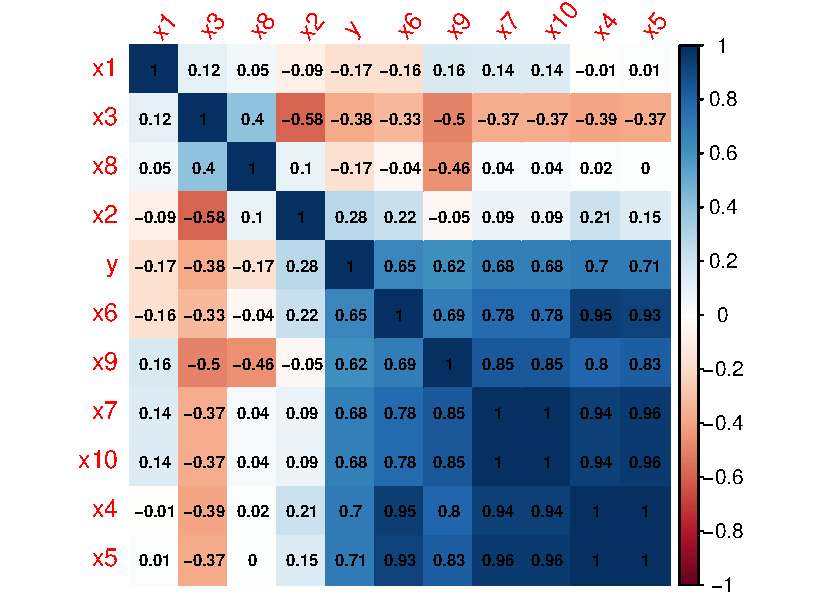
\includegraphics{lista2_files/figure-pdf/unnamed-chunk-3-1.pdf}

}

\caption{Correlograma das variáveis disponíveis}

\end{figure}

\begin{figure}

{\centering 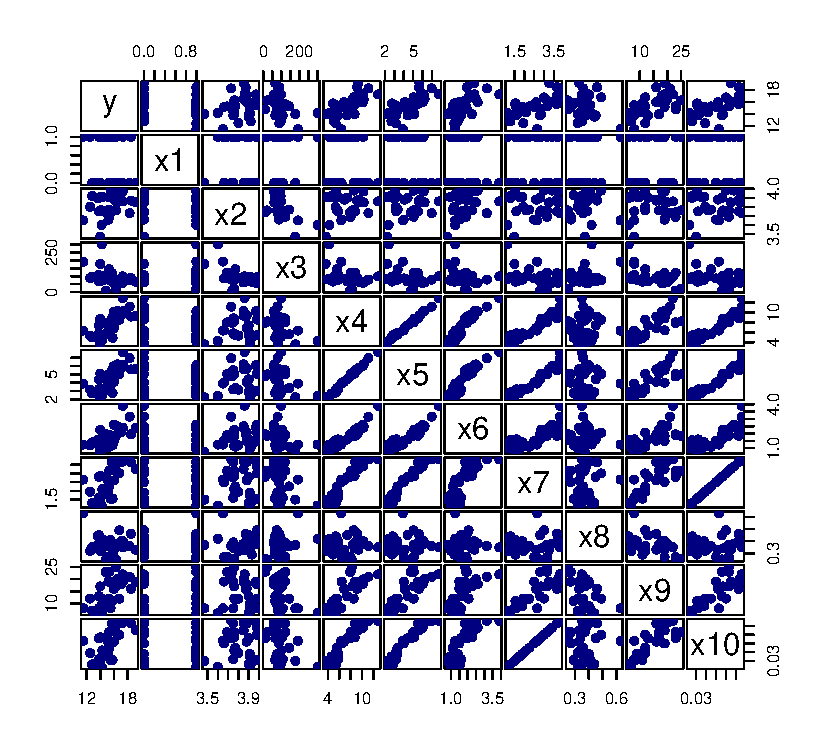
\includegraphics{lista2_files/figure-pdf/unnamed-chunk-4-1.pdf}

}

\caption{Correlações dois a dois das variáveis disponíveis.}

\end{figure}

\newpage{}

Nota-se a partir dos gráficos apresentados que:

\begin{itemize}
  \item A variável x1 tem apenas correlações fracas;
  \item A variável x2 tem apenas uma correlação negativa moderada com x3;
  \item A variável x3 tem correlação moderada com todas as variáveis, exceto com x1;
  \item A variável x4 tem correlação forte positiva com y, x5, x6, x7, x9, x10, além de uma correlação moderada negativa com x3;
  \item A variável x5 tem correlação forte positiva com y, x4, x6, x7, x9, x10, além de uma correlação moderada negativa com x3;
  \item A variável x6 tem correlação forte positiva com y, x4, x5, x7, x10, além de uma correlação moderada negativa e positiva com, respectivamente, x3 e x9;
  \item A variável x7 tem correlação forte positiva com x4, x5, x6, x9, correlação moderada negativa e positiva com, respectivamente, x3 e y, além de uma correlação perfeita com x10;
  \item A variável x8 tem apenas correlação moderada positiva e negativa, respectivamente, com x3 e x9;
  \item A variável x9 tem correlação forte positiva com x4, x5, x7, x10, além de uma correlação moderada positiva com y e x6 e negativa com x3 e x8;
  \item A variável x10 tem correlação forte positiva com x4, x5, x6, x9, correlação moderada positiva com y e negativa com x3, além de uma correlação perfeita com x7.
\end{itemize}

Independentemente das correlações, vamos aplicar um modelo de regressão
linear múltiplo completo, com todas as variáveis, para analisar e
modelar a relação entre a variável dependente ou resposta \(y\) e as
variáveis independentes ou explicativas
\(x_i \ \forall \ i = \{ 1,2,\dots,10 \}\).

\begin{longtable}[t]{lcccc}
\caption{Modelo de regressão linear múltipla completo, aplicado para todas as variáveis.}\\
\toprule
Coeficiente & Estimativa & EP & Estatística t & p-valor\\
\midrule
\endfirsthead
\caption[]{Modelo de regressão linear múltipla completo, aplicado para todas as variáveis. \textit{(continued)}}\\
\toprule
Coeficiente & Estimativa & EP & Estatística t & p-valor\\
\midrule
\endhead

\endfoot
\bottomrule
\endlastfoot
\cellcolor{gray!15}{(Intercept)} & \cellcolor{gray!15}{-12.208} & \cellcolor{gray!15}{14.612} & \cellcolor{gray!15}{-0.836} & \cellcolor{gray!15}{0.412}\\
x1 & -0.846 & 0.586 & -1.443 & 0.162\\
\cellcolor{gray!15}{x2} & \cellcolor{gray!15}{7.418} & \cellcolor{gray!15}{3.512} & \cellcolor{gray!15}{2.112} & \cellcolor{gray!15}{0.046}\\
x3 & 0.010 & 0.009 & 1.220 & 0.235\\
\cellcolor{gray!15}{x4} & \cellcolor{gray!15}{-1.947} & \cellcolor{gray!15}{2.221} & \cellcolor{gray!15}{-0.877} & \cellcolor{gray!15}{0.390}\\
x5 & 4.895 & 3.218 & 1.521 & 0.142\\
\cellcolor{gray!15}{x6} & \cellcolor{gray!15}{-1.434} & \cellcolor{gray!15}{1.813} & \cellcolor{gray!15}{-0.791} & \cellcolor{gray!15}{0.437}\\
x8 & -11.425 & 7.881 & -1.450 & 0.161\\
\cellcolor{gray!15}{x9} & \cellcolor{gray!15}{-0.108} & \cellcolor{gray!15}{0.220} & \cellcolor{gray!15}{-0.490} & \cellcolor{gray!15}{0.629}\\*
\end{longtable}

Nota-se que duas variáveis, x7 e x10, apresentam estimadores no modelo
como \texttt{NA}. Isso contece porque há um elevado grau de correlação
entre elas, o que atrapalha na estimação dos parâmetros de ambas com
relação a variável resposta \(y\).

Ignorando por enquanto esse fato, podemos fazer uma análise prévia dos
resíduos desse modelo e averiguar se há alguma inconsistência. Para tal,
faz-se uma análise gráfica dos e, posteriormente, um teste de
normalidade dos resíduos e de autocorrelação entre os resíduos, além de
um teste de heterocedasticidade do modelo.

Analisando os gráficos a seguir, nota-se do primeiro gráfico que a linha
está aproximadamente horizontal. Logo, tem-se linearidade no modelo. No
segundo gráfico vê-se que os resíduos aparentam ter distribuição normal.
Já no terceiro gráfico, aparenta-se haver homocedasticidade, pois os
resíduos estão dispersos como retângulo. Por fim, no quarto gráfico,
para observar outliers e pontos influentes, não aparenta possuir
resíduos outliers pois os resíduos estão entre -3 e +3.

\begin{figure}

{\centering 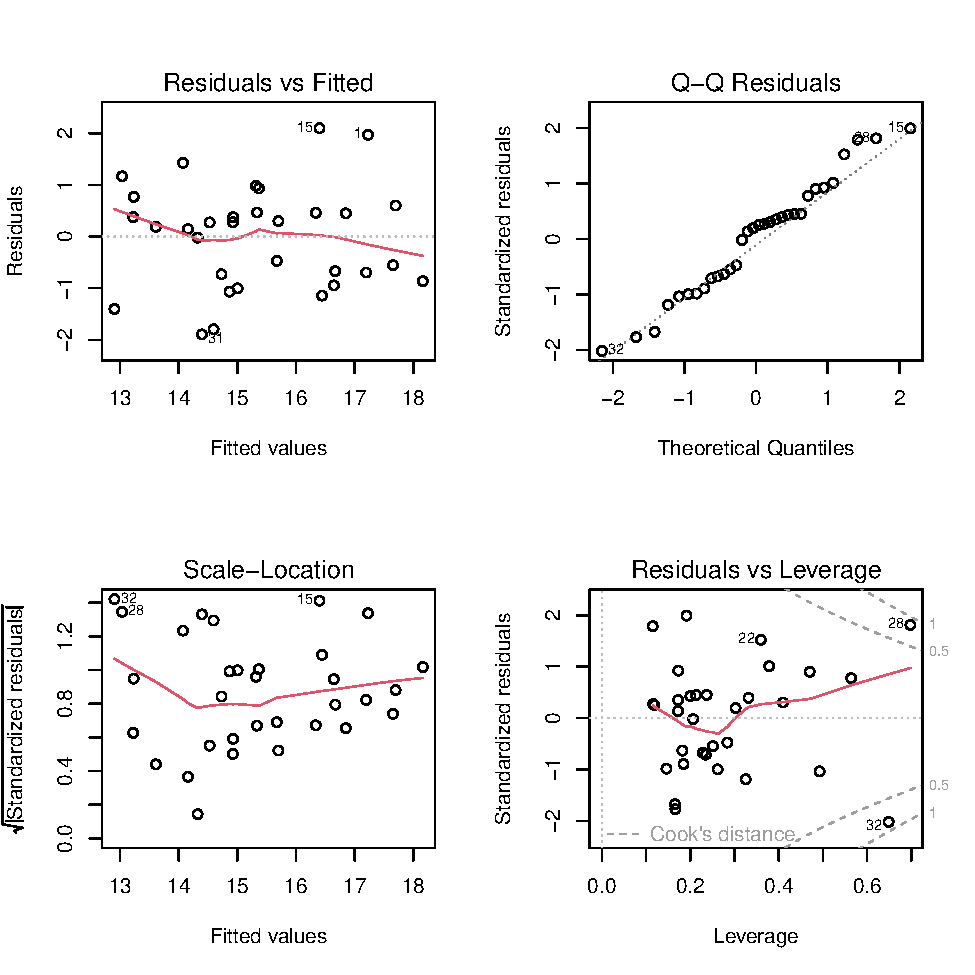
\includegraphics{lista2_files/figure-pdf/unnamed-chunk-6-1.pdf}

}

\end{figure}

Considerando os testes aplicados, nota-se que não há outliers nos
resíduos, não rejeita-se normalidade dos resíduos, não há evidências de
que há heterocedasticidade e não rejeita-se a independência dos
resíduos, logo, eles não apresentam autocorrelação.

\begin{longtable}[t]{cccccc}
\caption{Medidas estatísticas dos resíduos do modelo completo.}\\
\toprule
minimum & q1 & median & mean & q3 & maximum\\
\midrule
\endfirsthead
\caption[]{Medidas estatísticas dos resíduos do modelo completo. \textit{(continued)}}\\
\toprule
minimum & q1 & median & mean & q3 & maximum\\
\midrule
\endhead

\endfoot
\bottomrule
\endlastfoot
\cellcolor{gray!15}{-2.02} & \cellcolor{gray!15}{-0.757} & \cellcolor{gray!15}{0.223} & \cellcolor{gray!15}{0.01} & \cellcolor{gray!15}{0.533} & \cellcolor{gray!15}{1.993}\\*
\end{longtable}

\begin{longtable}[t]{lcc}
\caption{Testes de hipótese para normalidade, heteroscedasticidade e independência.}\\
\toprule
Teste & Estatística de teste & p-valor\\
\midrule
\endfirsthead
\caption[]{Testes de hipótese para normalidade, heteroscedasticidade e independência. \textit{(continued)}}\\
\toprule
Teste & Estatística de teste & p-valor\\
\midrule
\endhead

\endfoot
\bottomrule
\endlastfoot
\cellcolor{gray!15}{Shapiro-Wilk normality test} & \cellcolor{gray!15}{0.974} & \cellcolor{gray!15}{0.615}\\
studentized Breusch-Pagan test & 3.036 & 0.932\\
\cellcolor{gray!15}{Durbin-Watson Test} & \cellcolor{gray!15}{1.973} & \cellcolor{gray!15}{0.792}\\*
\end{longtable}

Já que os resíduos aparentam seguir as características esperadas, vamos
avaliar se há multicolinearidade no modelo, uma vez que haviam fortes
correlações entre as variáveis.

\newpage{}

\hypertarget{a-proponha-algum-muxe9todo-para-resolver-o-problema-da-multicolinearidade-no-conjunto-de-dados}{%
\subsection{a) Proponha algum método para resolver o problema da
multicolinearidade no conjunto de
dados}\label{a-proponha-algum-muxe9todo-para-resolver-o-problema-da-multicolinearidade-no-conjunto-de-dados}}

Nota-se do tópico anterior que x7 e x10 são fortemente correlacionadas
com outras variáveis, o que impossibilita de se estimar os parâmetros
dessas variáveis para o modelo. Logo, podemos retirá-las e analisar
novamente o modelo, avaliando se ainda há multicolinearidade nele por
meio da medida VIF, calculada para cada variável.

\begin{longtable}[t]{lcccc}
\caption{Modelo de regressão linear sem x7 e x10}\\
\toprule
Coeficiente & Estimativa & EP & Estatística t & p-valor\\
\midrule
\endfirsthead
\caption[]{Modelo de regressão linear sem x7 e x10 \textit{(continued)}}\\
\toprule
Coeficiente & Estimativa & EP & Estatística t & p-valor\\
\midrule
\endhead

\endfoot
\bottomrule
\endlastfoot
\cellcolor{gray!15}{(Intercept)} & \cellcolor{gray!15}{-12.208} & \cellcolor{gray!15}{14.612} & \cellcolor{gray!15}{-0.836} & \cellcolor{gray!15}{0.412}\\
x1 & -0.846 & 0.586 & -1.443 & 0.162\\
\cellcolor{gray!15}{x2} & \cellcolor{gray!15}{7.418} & \cellcolor{gray!15}{3.512} & \cellcolor{gray!15}{2.112} & \cellcolor{gray!15}{0.046}\\
x3 & 0.010 & 0.009 & 1.220 & 0.235\\
\cellcolor{gray!15}{x4} & \cellcolor{gray!15}{-1.947} & \cellcolor{gray!15}{2.221} & \cellcolor{gray!15}{-0.877} & \cellcolor{gray!15}{0.390}\\
x5 & 4.895 & 3.218 & 1.521 & 0.142\\
\cellcolor{gray!15}{x6} & \cellcolor{gray!15}{-1.434} & \cellcolor{gray!15}{1.813} & \cellcolor{gray!15}{-0.791} & \cellcolor{gray!15}{0.437}\\
x8 & -11.425 & 7.881 & -1.450 & 0.161\\
\cellcolor{gray!15}{x9} & \cellcolor{gray!15}{-0.108} & \cellcolor{gray!15}{0.220} & \cellcolor{gray!15}{-0.490} & \cellcolor{gray!15}{0.629}\\*
\end{longtable}

\begin{longtable}[t]{cc}
\caption{VIF para modelo sem x7 e x10}\\
\toprule
Variável & VIF\\
\midrule
\endfirsthead
\caption[]{VIF para modelo sem x7 e x10 \textit{(continued)}}\\
\toprule
Variável & VIF\\
\midrule
\endhead

\endfoot
\bottomrule
\endlastfoot
\cellcolor{gray!15}{x1} & \cellcolor{gray!15}{1.971}\\
x2 & 4.092\\
\cellcolor{gray!15}{x3} & \cellcolor{gray!15}{4.513}\\
x4 & 603.519\\
\cellcolor{gray!15}{x5} & \cellcolor{gray!15}{511.870}\\
x6 & 33.320\\
\cellcolor{gray!15}{x8} & \cellcolor{gray!15}{7.931}\\
x9 & 36.171\\*
\end{longtable}

Analisando os VIFs, nota-se que apesar de se retirar x7 e x10 ainda há
multicolinearidade no modelo. Poderíamos agora testar três métodos para
se retirar a multicolinearidade, sem precisar retirar as variáveis:
centrar, escalonar ou padronizar empiricamente as variáveis preditoras.
No entanto, após testar os três métodos, percebeu-se que não mudou os
índices de multicolinearidade. Logo, esses métodos não foram eficazes.
Portanto, testaremos a remoção da variável de maior VIF, x4.

\begin{longtable}[t]{lcccc}
\caption{Modelo de regressão linear sem x4, x7 e x10}\\
\toprule
Coeficiente & Estimativa & EP & Estatística t & p-valor\\
\midrule
\endfirsthead
\caption[]{Modelo de regressão linear sem x4, x7 e x10 \textit{(continued)}}\\
\toprule
Coeficiente & Estimativa & EP & Estatística t & p-valor\\
\midrule
\endhead

\endfoot
\bottomrule
\endlastfoot
\cellcolor{gray!15}{(Intercept)} & \cellcolor{gray!15}{-8.931} & \cellcolor{gray!15}{14.057} & \cellcolor{gray!15}{-0.635} & \cellcolor{gray!15}{0.531}\\
x1 & -1.008 & 0.553 & -1.821 & 0.081\\
\cellcolor{gray!15}{x2} & \cellcolor{gray!15}{6.267} & \cellcolor{gray!15}{3.242} & \cellcolor{gray!15}{1.933} & \cellcolor{gray!15}{0.065}\\
x3 & 0.013 & 0.008 & 1.550 & 0.134\\
\cellcolor{gray!15}{x5} & \cellcolor{gray!15}{2.250} & \cellcolor{gray!15}{1.115} & \cellcolor{gray!15}{2.017} & \cellcolor{gray!15}{0.055}\\
x6 & -2.517 & 1.320 & -1.907 & 0.069\\
\cellcolor{gray!15}{x8} & \cellcolor{gray!15}{-11.994} & \cellcolor{gray!15}{7.816} & \cellcolor{gray!15}{-1.534} & \cellcolor{gray!15}{0.138}\\
x9 & -0.079 & 0.217 & -0.365 & 0.718\\*
\end{longtable}

\begin{longtable}[t]{cc}
\caption{VIF para modelo sem x4, x7 e x10}\\
\toprule
Variável & VIF\\
\midrule
\endfirsthead
\caption[]{VIF para modelo sem x4, x7 e x10 \textit{(continued)}}\\
\toprule
Variável & VIF\\
\midrule
\endhead

\endfoot
\bottomrule
\endlastfoot
\cellcolor{gray!15}{x1} & \cellcolor{gray!15}{1.775}\\
x2 & 3.520\\
\cellcolor{gray!15}{x3} & \cellcolor{gray!15}{4.131}\\
x5 & 62.068\\
\cellcolor{gray!15}{x6} & \cellcolor{gray!15}{17.840}\\
x8 & 7.877\\
\cellcolor{gray!15}{x9} & \cellcolor{gray!15}{35.369}\\*
\end{longtable}

Ainda notando-se alta multicolinearidade, podemos eliminar a variável x5
de maior VIF, ou seja, maior grau de correlação com as demais, e
analisar o que acontece.

\begin{longtable}[t]{lcccc}
\caption{Modelo de regressão linear sem x4, x5, x7 e x10}\\
\toprule
Coeficiente & Estimativa & EP & Estatística t & p-valor\\
\midrule
\endfirsthead
\caption[]{Modelo de regressão linear sem x4, x5, x7 e x10 \textit{(continued)}}\\
\toprule
Coeficiente & Estimativa & EP & Estatística t & p-valor\\
\midrule
\endhead

\endfoot
\bottomrule
\endlastfoot
\cellcolor{gray!15}{(Intercept)} & \cellcolor{gray!15}{-21.075} & \cellcolor{gray!15}{13.460} & \cellcolor{gray!15}{-1.566} & \cellcolor{gray!15}{0.130}\\
x1 & -1.235 & 0.574 & -2.150 & 0.041\\
\cellcolor{gray!15}{x2} & \cellcolor{gray!15}{8.114} & \cellcolor{gray!15}{3.295} & \cellcolor{gray!15}{2.462} & \cellcolor{gray!15}{0.021}\\
x3 & 0.015 & 0.009 & 1.695 & 0.102\\
\cellcolor{gray!15}{x6} & \cellcolor{gray!15}{-0.211} & \cellcolor{gray!15}{0.700} & \cellcolor{gray!15}{-0.302} & \cellcolor{gray!15}{0.765}\\
x8 & 1.827 & 3.987 & 0.458 & 0.651\\
\cellcolor{gray!15}{x9} & \cellcolor{gray!15}{0.310} & \cellcolor{gray!15}{0.105} & \cellcolor{gray!15}{2.953} & \cellcolor{gray!15}{0.007}\\*
\end{longtable}

\begin{longtable}[t]{cc}
\caption{VIF para modelo sem x4, x5, x7 e x10}\\
\toprule
Variável & VIF\\
\midrule
\endfirsthead
\caption[]{VIF para modelo sem x4, x5, x7 e x10 \textit{(continued)}}\\
\toprule
Variável & VIF\\
\midrule
\endhead

\endfoot
\bottomrule
\endlastfoot
\cellcolor{gray!15}{x1} & \cellcolor{gray!15}{1.702}\\
x2 & 3.239\\
\cellcolor{gray!15}{x3} & \cellcolor{gray!15}{4.076}\\
x6 & 4.463\\
\cellcolor{gray!15}{x8} & \cellcolor{gray!15}{1.826}\\
x9 & 7.379\\*
\end{longtable}

Agora sim foi possível eliminar a multicolinearidade e seguir para uma
seleção do melhor modelo final.

\hypertarget{b-usando-algum-muxe9todo-de-seleuxe7uxe3o-de-variuxe1veis-obtenha-o-modelo-final-para-o-conjunto-de-dados}{%
\subsection{b) Usando algum método de seleção de variáveis, obtenha o
modelo final para o conjunto de
dados}\label{b-usando-algum-muxe9todo-de-seleuxe7uxe3o-de-variuxe1veis-obtenha-o-modelo-final-para-o-conjunto-de-dados}}

Considerando os métodos de seleção de variáveis Forward, Bacward e
Stepwise, pode-se selecionar o melhor modelo com base no critério de
AIC.

Pelo método de seleção de variáveis \emph{stepwise backward}, obtém-se o
melhor modelo, com menor AIC (Critério de Informação de Akaike), no
formato
\(\hat{y}_i = \hat{\beta}_0 + \hat{\beta}_1 \, x_{1i} + \hat{\beta}_2 \,x_{2i} + \hat{\beta}_3 \, x_{3i} + \hat{\beta}_9\,x_{9i}\),
excluindo-se as vaiáveis x4, x5, x6, x7, x8, x10 do modelo.

\begin{longtable}[t]{lcccc}
\caption{Modelo de regressão linear com x1, x2, x3 e x9}\\
\toprule
Coeficiente & Estimativa & EP & Estatística t & p-valor\\
\midrule
\endfirsthead
\caption[]{Modelo de regressão linear com x1, x2, x3 e x9 \textit{(continued)}}\\
\toprule
Coeficiente & Estimativa & EP & Estatística t & p-valor\\
\midrule
\endhead

\endfoot
\bottomrule
\endlastfoot
\cellcolor{gray!15}{(Intercept)} & \cellcolor{gray!15}{-19.615} & \cellcolor{gray!15}{10.347} & \cellcolor{gray!15}{-1.896} & \cellcolor{gray!15}{0.069}\\
x1 & -1.122 & 0.446 & -2.516 & 0.018\\
\cellcolor{gray!15}{x2} & \cellcolor{gray!15}{7.911} & \cellcolor{gray!15}{2.494} & \cellcolor{gray!15}{3.172} & \cellcolor{gray!15}{0.004}\\
x3 & 0.014 & 0.007 & 2.118 & 0.043\\
\cellcolor{gray!15}{x9} & \cellcolor{gray!15}{0.280} & \cellcolor{gray!15}{0.051} & \cellcolor{gray!15}{5.488} & \cellcolor{gray!15}{0.000}\\*
\end{longtable}

\begin{longtable}[t]{cc}
\caption{VIF para modelo linear com x1, x2, x3 e x9}\\
\toprule
Variável & VIF\\
\midrule
\endfirsthead
\caption[]{VIF para modelo linear com x1, x2, x3 e x9 \textit{(continued)}}\\
\toprule
Variável & VIF\\
\midrule
\endhead

\endfoot
\bottomrule
\endlastfoot
\cellcolor{gray!15}{x1} & \cellcolor{gray!15}{1.098}\\
x2 & 1.986\\
\cellcolor{gray!15}{x3} & \cellcolor{gray!15}{2.754}\\
x9 & 1.862\\*
\end{longtable}

Com isso, seleciona-se o seguinte modelo final, com todas as variáveis
significativas e sem multicolinearidade:

\begin{align}
  y_i = \beta_0 + \beta_1 \, x_{i1} + \beta_2 \, x_{i2} + \beta_3 \, x_{i3}\ + \beta_4 \, x_{i9} + \varepsilon_i, \quad i = 1, 2, \dots, 32.
\end{align}

\hypertarget{c-apresente-a-tabela-de-anuxe1lise-de-variuxe2ncia-para-testar-a-significuxe2ncia-global-dos-coeficientes-do-modelo-final.-apresente-as-hipuxf3teses-de-teste-e-conclua.}{%
\subsection{c) Apresente a tabela de Análise de Variância para testar a
significância global dos coeficientes do modelo final. Apresente as
hipóteses de teste e
conclua.}\label{c-apresente-a-tabela-de-anuxe1lise-de-variuxe2ncia-para-testar-a-significuxe2ncia-global-dos-coeficientes-do-modelo-final.-apresente-as-hipuxf3teses-de-teste-e-conclua.}}

Para testar as hipóteses

\begin{align}
  H_0: \beta_j = 0, \quad H_a: \beta_j \neq 0
\end{align}

monta-se a seguinte tabela de análise de variância:

\begin{longtable}[t]{lccccl}
\caption{Tabela ANOVA para o modelo linear com x1, x2, x2, x3 e x9}\\
\toprule
Fonte de Var. & g.l. & SQ & QM & F & p-valor\\
\midrule
\endfirsthead
\caption[]{Tabela ANOVA para o modelo linear com x1, x2, x2, x3 e x9 \textit{(continued)}}\\
\toprule
Fonte de Var. & g.l. & SQ & QM & F & p-valor\\
\midrule
\endhead

\endfoot
\bottomrule
\endlastfoot
\cellcolor{gray!15}{x1} & \cellcolor{gray!15}{1} & \cellcolor{gray!15}{2.805} & \cellcolor{gray!15}{2.805} & \cellcolor{gray!15}{1.968} & \cellcolor{gray!15}{0.172}\\
x2 & 1 & 6.745 & 6.745 & 4.732 & 0.039\\
\cellcolor{gray!15}{x3} & \cellcolor{gray!15}{1} & \cellcolor{gray!15}{6.223} & \cellcolor{gray!15}{6.223} & \cellcolor{gray!15}{4.365} & \cellcolor{gray!15}{0.046}\\
x9 & 1 & 42.940 & 42.940 & 30.123 & 0.000\\
\cellcolor{gray!15}{Residuals} & \cellcolor{gray!15}{27} & \cellcolor{gray!15}{38.488} & \cellcolor{gray!15}{1.425} & \cellcolor{gray!15}{NA} & \cellcolor{gray!15}{NA}\\*
\end{longtable}

Pode-se concluir que para um nível de significância de 0.05, a variável
x1 não tem seu coeficiente significativamente diferente de zero para o
modelo, o que significa que pode-se considerar a sua remoção. Isto é,
essa variável não contribui de forma estatisticamente significativa para
a explicação da variável \(y\). Dessa forma, analisa-se novamente a
ANOVA.

Nota-se ainda que, ao retirar x1, x3 também passa a não contribuir de
forma estatisticamente significativa para a explicação da variável
\(y\), apresentando coeficiente significativamente igual a 0 para um
nível de significância de 0,05. Logo, retira-se essa variável também.

\begin{longtable}[t]{lcccc}
\caption{Modelo de regressão linear com x2, x3 e x9}\\
\toprule
Coeficiente & Estimativa & EP & Estatística t & p-valor\\
\midrule
\endfirsthead
\caption[]{Modelo de regressão linear com x2, x3 e x9 \textit{(continued)}}\\
\toprule
Coeficiente & Estimativa & EP & Estatística t & p-valor\\
\midrule
\endhead

\endfoot
\bottomrule
\endlastfoot
\cellcolor{gray!15}{(Intercept)} & \cellcolor{gray!15}{-16.652} & \cellcolor{gray!15}{11.215} & \cellcolor{gray!15}{-1.485} & \cellcolor{gray!15}{0.149}\\
x2 & 7.206 & 2.704 & 2.665 & 0.013\\
\cellcolor{gray!15}{x3} & \cellcolor{gray!15}{0.010} & \cellcolor{gray!15}{0.007} & \cellcolor{gray!15}{1.428} & \cellcolor{gray!15}{0.164}\\
x9 & 0.244 & 0.053 & 4.571 & 0.000\\*
\end{longtable}

\begin{longtable}[t]{lccccl}
\caption{Tabela ANOVA para o modelo linear com x2, x3 e x9}\\
\toprule
Fonte de Var. & g.l. & SQ & QM & F & p-valor\\
\midrule
\endfirsthead
\caption[]{Tabela ANOVA para o modelo linear com x2, x3 e x9 \textit{(continued)}}\\
\toprule
Fonte de Var. & g.l. & SQ & QM & F & p-valor\\
\midrule
\endhead

\endfoot
\bottomrule
\endlastfoot
\cellcolor{gray!15}{x2} & \cellcolor{gray!15}{1} & \cellcolor{gray!15}{7.483} & \cellcolor{gray!15}{7.483} & \cellcolor{gray!15}{4.410} & \cellcolor{gray!15}{0.045}\\
x3 & 1 & 6.757 & 6.757 & 3.982 & 0.056\\
\cellcolor{gray!15}{x9} & \cellcolor{gray!15}{1} & \cellcolor{gray!15}{35.450} & \cellcolor{gray!15}{35.450} & \cellcolor{gray!15}{20.892} & \cellcolor{gray!15}{0.000}\\
Residuals & 28 & 47.510 & 1.697 & NA & NA\\*
\end{longtable}

Por fim, para \(\alpha = 0.05\), temos o modelo final para esses dados,
que é

\begin{align}
  y_i = \beta_0 + \beta_1 \, x_{i2} + \beta_2 \, x_{i9} + \varepsilon_i, \quad i = 1, 2, \dots, 32,
\end{align}

obtido considerando os resultados das tabelas a seguir.

\begin{longtable}[t]{lcccc}
\caption{Modelo de regressão linear com x2 e x9}\\
\toprule
Coeficiente & Estimativa & EP & Estatística t & p-valor\\
\midrule
\endfirsthead
\caption[]{Modelo de regressão linear com x2 e x9 \textit{(continued)}}\\
\toprule
Coeficiente & Estimativa & EP & Estatística t & p-valor\\
\midrule
\endhead

\endfoot
\bottomrule
\endlastfoot
\cellcolor{gray!15}{(Intercept)} & \cellcolor{gray!15}{-4.660} & \cellcolor{gray!15}{7.566} & \cellcolor{gray!15}{-0.616} & \cellcolor{gray!15}{0.543}\\
x2 & 4.507 & 1.968 & 2.291 & 0.029\\
\cellcolor{gray!15}{x9} & \cellcolor{gray!15}{0.195} & \cellcolor{gray!15}{0.042} & \cellcolor{gray!15}{4.695} & \cellcolor{gray!15}{0.000}\\*
\end{longtable}

\begin{longtable}[t]{lccccl}
\caption{Tabela ANOVA para o modelo linear com x2 e x9}\\
\toprule
Fonte de Var. & g.l. & SQ & QM & F & p-valor\\
\midrule
\endfirsthead
\caption[]{Tabela ANOVA para o modelo linear com x2 e x9 \textit{(continued)}}\\
\toprule
Fonte de Var. & g.l. & SQ & QM & F & p-valor\\
\midrule
\endhead

\endfoot
\bottomrule
\endlastfoot
\cellcolor{gray!15}{x2} & \cellcolor{gray!15}{1} & \cellcolor{gray!15}{7.483} & \cellcolor{gray!15}{7.483} & \cellcolor{gray!15}{4.258} & \cellcolor{gray!15}{0.048}\\
x9 & 1 & 38.747 & 38.747 & 22.045 & 0.000\\
\cellcolor{gray!15}{Residuals} & \cellcolor{gray!15}{29} & \cellcolor{gray!15}{50.970} & \cellcolor{gray!15}{1.758} & \cellcolor{gray!15}{NA} & \cellcolor{gray!15}{NA}\\*
\end{longtable}

\hypertarget{d-com-base-no-modelo-obtido-no-item-anterior-fauxe7a-uma-anuxe1lise-de-resuxedduos-e-conclua.}{%
\subsection{d) Com base no modelo obtido no item anterior, faça uma
análise de resíduos e
conclua.}\label{d-com-base-no-modelo-obtido-no-item-anterior-fauxe7a-uma-anuxe1lise-de-resuxedduos-e-conclua.}}

Para uma análise de resíduos, fazemos uma análise gráfica e,
posteriormente, teste de normalidade, de autocorrelação e de
heterocedasticidade do dos resíduos.

Analisando os gráficos, nota-se que estão aproximadamente distribuídos
em torno de zero, que os resíduos apresentam ter distribuição normal,
que aparenta-se haver homocedasticidade e que não aparenta possuir
resíduos outliers.

\begin{figure}

{\centering 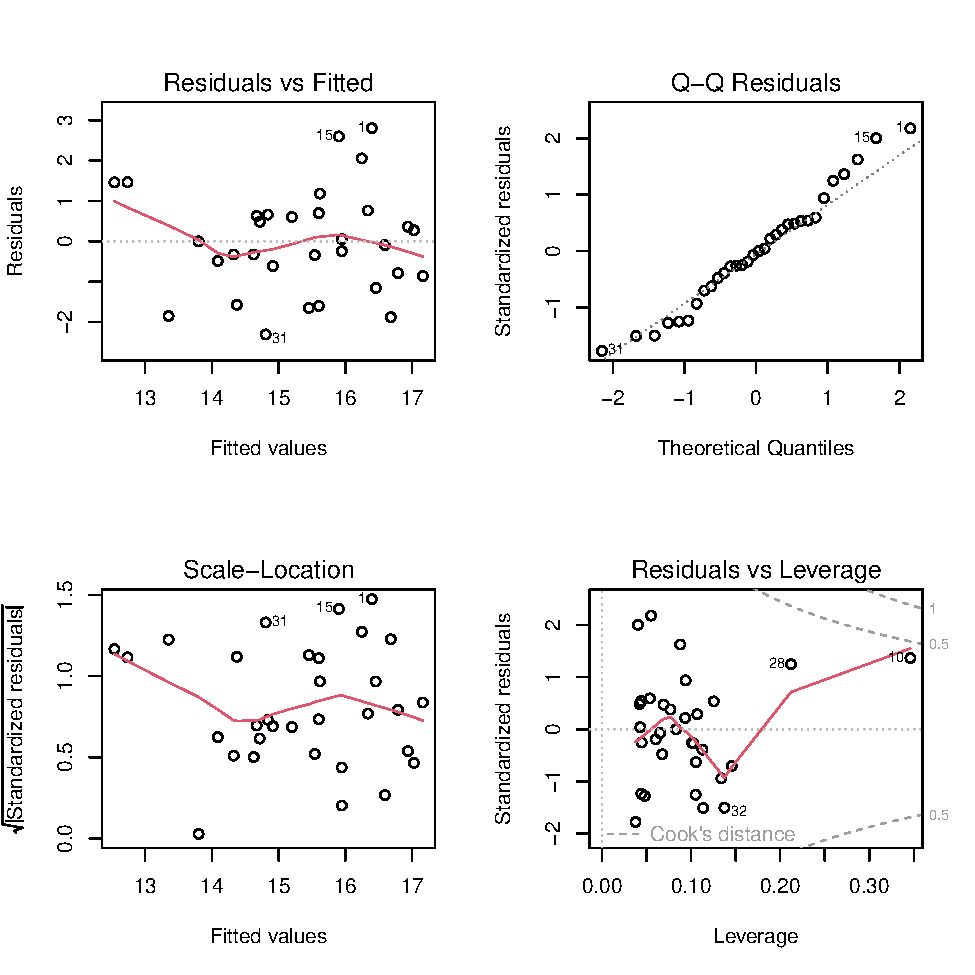
\includegraphics{lista2_files/figure-pdf/unnamed-chunk-17-1.pdf}

}

\end{figure}

Confirmando as informações gráficas através dos testes, para um nível de
significância de 0,05, nota-se que não há outliers nos resíduos, não
rejeita-se normalidade dos resíduos, não há evidências de que há
heterocedasticidade e não rejeita-se a independência dos resíduos, logo,
eles não apresentam autocorrelação.

\begin{longtable}[t]{lcc}
\caption{Testes de hipótese para normalidade, heteroscedasticidade e independência.}\\
\toprule
Teste & Estatística de teste & p-valor\\
\midrule
\endfirsthead
\caption[]{Testes de hipótese para normalidade, heteroscedasticidade e independência. \textit{(continued)}}\\
\toprule
Teste & Estatística de teste & p-valor\\
\midrule
\endhead

\endfoot
\bottomrule
\endlastfoot
\cellcolor{gray!15}{Shapiro-Wilk normality test} & \cellcolor{gray!15}{0.977} & \cellcolor{gray!15}{0.697}\\
studentized Breusch-Pagan test & 1.067 & 0.587\\
\cellcolor{gray!15}{Durbin-Watson Test} & \cellcolor{gray!15}{1.421} & \cellcolor{gray!15}{0.090}\\*
\end{longtable}

\begin{longtable}[t]{lcclcc}
\caption{Medidas descritivas dos resíduos padronizados.}\\
\toprule
minimum & q1 & median & mean & q3 & maximum\\
\midrule
\endfirsthead
\caption[]{Medidas descritivas dos resíduos padronizados. \textit{(continued)}}\\
\toprule
minimum & q1 & median & mean & q3 & maximum\\
\midrule
\endhead

\endfoot
\bottomrule
\endlastfoot
\cellcolor{gray!15}{-1.773} & \cellcolor{gray!15}{-0.646} & \cellcolor{gray!15}{-0.036} & \cellcolor{gray!15}{0.005} & \cellcolor{gray!15}{0.536} & \cellcolor{gray!15}{2.176}\\*
\end{longtable}

Portanto, como os resíduos estão de acordo com as suposições esperadas,
pode-se concluir que o modelo escolhido no item anterior como modelo
final, com a relação entre \(y\), x2 e x9, está adequado. Fazendo uma
análise desse modelo de regressão linear múltipla, poderia-se afirmar
que para cada 1 unidade a mais de PH do vinho, a qualidade do vinho
aumentaria, em média, 4.5 (t= 2.291; p-valor = 0.0294). Já para cada
aumento de um grau de ionização das antocianinas (em porcentagem), a
qualidade do vinho aumentaria, em média, 0.19 (t= 4.695; p-valor =
5.91e-05).

\newpage{}

\hypertarget{questuxe3o-2}{%
\section{Questão 2}\label{questuxe3o-2}}

Uma equipe de pesquisadores de saúde mental deseja comparar três métodos
de tratamento da depressão grave (A, B e C=referência). Eles também
gostariam de estudara relação entre idade e eficácia do tratamento, bem
como a interação (se houver) entre idade e tratamento. Cada elemento da
amostra aleatória simples de 36 pacientes, foi selecionado
aleatoriamente para receber o tratamento A, B ou C. Os dados obtidos
podem ser encontrados no ficheiro \texttt{Q02-data.txt}. A variável
dependente \(y\) é a eficácia do tratamento; as variáveis independentes
são: a idade do paciente no aniversário mais próximo e o tipo de
tratamento administrado (use 1\% de significância durantes as análises).

Uma amostra dos dados é exibida na tabela a seguir:

\begin{longtable*}{ccc}
\toprule
eficacia & idade & tratamento\\
\midrule
\endfirsthead
\multicolumn{3}{@{}l}{\textit{(continued)}}\\
\toprule
eficacia & idade & tratamento\\
\midrule
\endhead

\endfoot
\bottomrule
\endlastfoot
\cellcolor{gray!15}{56} & \cellcolor{gray!15}{21} & \cellcolor{gray!15}{A}\\
41 & 23 & B\\
\cellcolor{gray!15}{40} & \cellcolor{gray!15}{30} & \cellcolor{gray!15}{B}\\
28 & 19 & C\\
\cellcolor{gray!15}{55} & \cellcolor{gray!15}{28} & \cellcolor{gray!15}{A}\\
25 & 23 & C\\*
\end{longtable*}

Um histograma da variável resposta é exibido a seguir, sugerindo
assimetria na sua distribuição.

\begin{figure}

{\centering 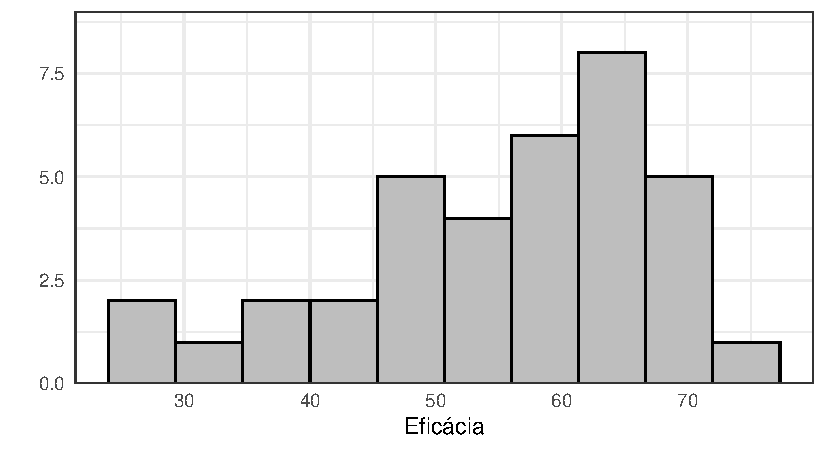
\includegraphics{lista2_files/figure-pdf/histograma-q2-1.pdf}

}

\caption{Histograma da variável resposta}

\end{figure}

No entanto, se montamos um histograma da variável resposta para cada
valor de tratamento, vemos que há uma discrepência na sua distribuição.
O tratamento A está bem concentrando em eficácias mais altas, enquanto o
B está mais concentrado ao centro da métrica de eficácia e o C está
amplamente distribuído.

\begin{figure}

{\centering 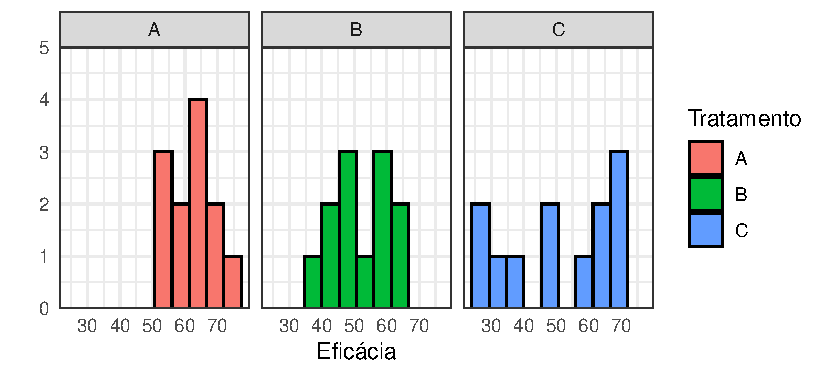
\includegraphics{lista2_files/figure-pdf/histograma-q2-facet-1.pdf}

}

\caption{Histograma da variável resposta segregado por tratamento}

\end{figure}

\hypertarget{a-ajuste-um-modelo-de-regressuxe3o-linear-e-interprete-os-resultados-obtidos}{%
\subsection{a) Ajuste um modelo de regressão linear e interprete os
resultados
obtidos}\label{a-ajuste-um-modelo-de-regressuxe3o-linear-e-interprete-os-resultados-obtidos}}

Inicialmente, consideremos apenas um gráfico de dispersão entre a
variável resposta e a única variável numérica, Idade. É possível notar
uma relação que pode ou não ser linear, mas também há indícios de
heteroscedasticidade. As demais variáveis são dicotômicas, então não há
necessidade de se montar dispersões para elas.

Além disso, se segregamos a dispersão por grupos de tratamento, notamos
que pode ser preferível um modelo que considere comportamentos de cada
grupo separadamente.

\begin{figure}

{\centering 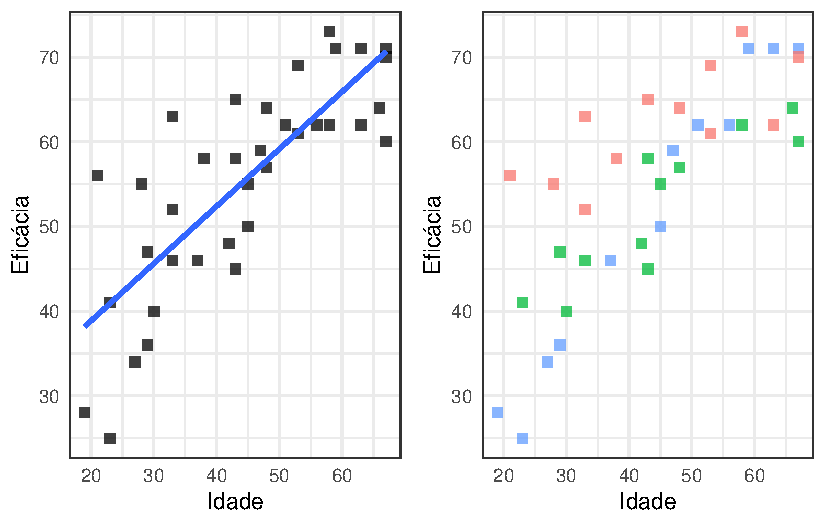
\includegraphics{lista2_files/figure-pdf/scatter-variaveis-1.pdf}

}

\caption{Gráficos de dispersão geral e segregado por tratamento}

\end{figure}

Temos um potencial modelo de regressão linear que pode ou não conter
interações entre as variáveis, o qual pode ser expresso em sua forma
saturada, em que \(X_1\) é a variável idade e \(X_2\) a variável
tratamento

\begin{align}
  y_i = \beta_0 + \beta_1 \, x_{1i} + \beta_2 \, x_{2i} + \beta_3 \, x_{1i}\, x_{2i} + \varepsilon_i, \quad i = 1, 2, \dots, n
\end{align}

ou, de forma análoga, desmembrando \(X_2\) em variáveis \emph{dummy}
\(X_A\) e \(X_B\), indicadores da presença do tratamento \(A\) e \(B\),
ambas assumindo valor \(0\) quando se trata do tratamento \(C\)

\begin{align}
  y_i = \beta_0 + \beta_1 \, x_{1i} + \beta_2 \, x_{Ai} + \beta_3 \, x_{Bi} + \beta_4 \, x_{1i} \, x_{Ai} + \beta_5 \, x_{1i} \, x_{Bi} + \varepsilon_i. \label{modelo_dummy}
\end{align}

Se simplesmente ajustamos um modelo de regressão linear -- sem os termos
de interação -- utilizando (\ref{modelo_dummy}) como referência na
função \texttt{lm()}, obtemos os seguintes resultados:

\begin{longtable}[t]{lcccc}
\caption{Modelo de regressão linear para tratamentos sem interação com idade sobre eficácia}\\
\toprule
Coeficiente & Estimativa & EP & Estatística t & p-valor\\
\midrule
\endfirsthead
\caption[]{Modelo de regressão linear para tratamentos sem interação com idade sobre eficácia \textit{(continued)}}\\
\toprule
Coeficiente & Estimativa & EP & Estatística t & p-valor\\
\midrule
\endhead

\endfoot
\bottomrule
\endlastfoot
\cellcolor{gray!15}{(Intercept)} & \cellcolor{gray!15}{22.291} & \cellcolor{gray!15}{3.505} & \cellcolor{gray!15}{6.359} & \cellcolor{gray!15}{0.000}\\
idade & 0.664 & 0.070 & 9.522 & 0.000\\
\cellcolor{gray!15}{A} & \cellcolor{gray!15}{10.253} & \cellcolor{gray!15}{2.465} & \cellcolor{gray!15}{4.159} & \cellcolor{gray!15}{0.000}\\
B & 0.445 & 2.464 & 0.181 & 0.858\\*
\end{longtable}

Ou seja, se considerarmos independentemente idade, tratamento A e
tratamento B, podemos considerar que:

\begin{itemize}
\tightlist
\item
  Há uma linha de base na eficácia de aproximadamente 22.3, i.e.~sob o
  tratamento C;
\item
  A eficácia base para o tratamento A é de 32.3;
\item
  A eficácia base para o tratamento B é de 22.75 -- mas poderíamos
  desconsiderar este coeficiente, se nos guiarmos pelo p-valor;
\item
  Cada ano a mais de vida incrementa a eficácia em 0.644.
\end{itemize}

É possível considerar que um tamanho de amostra pequeno tenha grande
influência sobre a significância de \(H_0: \beta_3 = 0\) do modelo. No
entanto, trata-se de um fenômeno para o qual o tratamento pode estar
estreitamente associado à idade, caso em que teríamos que considerar o
modelo (\ref{modelo_dummy}) por completo.

\hypertarget{b-obtenha-a-tabela-anova-para-o-modelo-obtido-no-item-a-e-interprete-os-resultados}{%
\subsection{b) Obtenha a tabela ANOVA para o modelo obtido no item (a) e
interprete os
resultados}\label{b-obtenha-a-tabela-anova-para-o-modelo-obtido-no-item-a-e-interprete-os-resultados}}

Se montarmos uma tabela de Análise de Variância para o modelo de
regressão linear ajustado, obtemos os resultados a seguir:

\begin{longtable}[t]{lccccl}
\caption{Tabela ANOVA para o modelo linear sem interações}\\
\toprule
Fonte de Var. & g.l. & SQ & QM & F & p-valor\\
\midrule
\endfirsthead
\caption[]{Tabela ANOVA para o modelo linear sem interações \textit{(continued)}}\\
\toprule
Fonte de Var. & g.l. & SQ & QM & F & p-valor\\
\midrule
\endhead

\endfoot
\bottomrule
\endlastfoot
\cellcolor{gray!15}{idade} & \cellcolor{gray!15}{1} & \cellcolor{gray!15}{3424.432} & \cellcolor{gray!15}{3424.432} & \cellcolor{gray!15}{94.015} & \cellcolor{gray!15}{0.000}\\
A & 1 & 803.804 & 803.804 & 22.068 & 0.000\\
\cellcolor{gray!15}{B} & \cellcolor{gray!15}{1} & \cellcolor{gray!15}{1.189} & \cellcolor{gray!15}{1.189} & \cellcolor{gray!15}{0.033} & \cellcolor{gray!15}{0.858}\\
Residuals & 32 & 1165.575 & 36.424 & NA & NA\\*
\end{longtable}

Nota-se que a maioria da variância explicada pelo modelo está associada
à variável idade, enquanto a soma de quadrados das variáveis de
tratamento juntas não superam a soma de quadrados dos resíduos.

Se conjugarmos os resultados deste item com os do item a) vemos que
isoladamente apenas idade, e interessantemente apenas o tratamento A,
parecem ser variáveis que realmente contribuem para a explicação do
fenômeno.

\hypertarget{c-considere-a-possibilidade-de-incluir-a-interauxe7uxe3o-entre-as-varuxe1veis-independentes}{%
\subsection{c) Considere a possibilidade de incluir a interação entre as
varáveis
independentes}\label{c-considere-a-possibilidade-de-incluir-a-interauxe7uxe3o-entre-as-varuxe1veis-independentes}}

\hypertarget{i-lista-de-todos-os-submodelos-possuxedveis}{%
\subsubsection{i) Lista de todos os submodelos
possíveis}\label{i-lista-de-todos-os-submodelos-possuxedveis}}

A partir do modelo (\ref{modelo_dummy}), construimos todos os possíveis
submodelos. Considerando que temos três covariáveis e dois termos de
interação, temos \(\sum\limits_{n = 1}^5\binom{6}{n} = 62\) modelos

\begin{enumerate}
  \item $y_i = \beta_0 + \varepsilon_i$
  \item $y_i = \beta_1 \, x_{1i} + \varepsilon_i$
  \item $y_i = \beta_2 \, x_{Ai} + \varepsilon_i$
  \item $y_i = \beta_3 \, x_{Bi} + \varepsilon_i$
  \item $y_i = \beta_4 \, x_{1i} \, x_{Ai} + \varepsilon_i$
  \item $y_i = \beta_5 \, x_{1i} \, x_{Bi} + \varepsilon_i$
  
 
  \item $y_i = \beta_0 + \beta_1 \, x_{1i} + \varepsilon_i$
  \item $y_i = \beta_0 + \beta_2 \, x_{Ai} + \varepsilon_i$
  \item $y_i = \beta_0 + \beta_3 \, x_{Bi} + \varepsilon_i$
  \item $y_i = \beta_0 + \beta_4 \, x_{1i} \, x_{Ai} + \varepsilon_i$
  \item $y_i = \beta_0 + \beta_5 \, x_{1i} \, x_{Bi} + \varepsilon_i$
  \item $y_i = \beta_1 \, x_{1i} + \beta_2 \, x_{Ai} + \varepsilon_i$
  \item $y_i = \beta_1 \, x_{1i} + \beta_3 \, x_{Bi} + \varepsilon_i$
  \item $y_i = \beta_1 \, x_{1i} + \beta_4 \, x_{1i} \, x_{Ai} + \varepsilon_i$
  \item $y_i =  \beta_1 \, x_{1i} + \beta_5 \, x_{1i} \, x_{Bi} + \varepsilon_i$
  \item $y_i = \beta_2 \, x_{Ai} + \beta_3 \, x_{Bi}+ \varepsilon_i$
  \item $y_i = \beta_2 \, x_{Ai} + \beta_4 \, x_{1i} \, x_{Ai} + \varepsilon_i$
  \item $y_i = \beta_2 \, x_{Ai} + \beta_5 \, x_{1i} \, x_{Bi} + \varepsilon_i$
  \item $y_i = \beta_3 \, x_{Bi} + \beta_4 \, x_{1i} \, x_{Ai} + \varepsilon_i$
  \item $y_i = \beta_3 \, x_{Bi} + \beta_5 \, x_{1i} \, x_{Bi} + \varepsilon_i$
  \item $y_i = \beta_4 \, x_{1i} \, x_{Ai} + \beta_5 \, x_{1i} \, x_{Bi} + \varepsilon_i$
  
  

  \item $y_i = \beta_0 + \beta_1 \, x_{1i} + \beta_2 \, x_{Ai} + \varepsilon_i$
  \item $y_i = \beta_0 + \beta_1 \, x_{1i} + \beta_3 \, x_{Bi} + \varepsilon_i$
  \item $y_i = \beta_0 + \beta_1 \, x_{1i} + \beta_4 \, x_{1i} \, x_{Ai} + \varepsilon_i$
  \item $y_i = \beta_0 + \beta_1 \, x_{1i} + \beta_5 \, x_{1i} \, x_{Bi} + \varepsilon_i$
  \item $y_i = \beta_0 + \beta_2 \, x_{Ai} + \beta_3 \, x_{Bi} + \varepsilon_i$
  \item $y_i = \beta_0 + \beta_2 \, x_{Ai} + \beta_4 \, x_{1i} \, x_{Ai} +  \varepsilon_i$
  \item $y_i = \beta_0 + \beta_2 \, x_{Ai} + \beta_5 \, x_{1i} \, x_{Bi} + \varepsilon_i$
  \item $y_i = \beta_0 + \beta_3 \, x_{Bi} + \beta_4 \, x_{1i} \, x_{Ai} +  \varepsilon_i$
  \item $y_i = \beta_0 + \beta_3 \, x_{Bi} + \beta_5 \, x_{1i} \, x_{Bi} + \varepsilon_i$
  \item $y_i = \beta_0 + \beta_4 \, x_{1i} \, x_{Ai} + \beta_5 \, x_{1i} \, x_{Bi} + \varepsilon_i$
  \item $y_i = \beta_1 \, x_{1i} + \beta_2 \, x_{Ai} + \beta_3 \, x_{Bi} + \varepsilon_i$
  \item $y_i = \beta_1 \, x_{1i} + \beta_2 \, x_{Ai} + \beta_4 \, x_{1i} \, x_{Ai} + \varepsilon_i$
  \item $y_i = \beta_1 \, x_{1i} + \beta_2 \, x_{Ai} + \beta_5 \, x_{1i} \, x_{Bi} + \varepsilon_i$
  \item $y_i = \beta_1 \, x_{1i} + \beta_3 \, x_{Bi} + \beta_4 \, x_{1i} \, x_{Ai} + \varepsilon_i$
  \item $y_i = \beta_1 \, x_{1i} + \beta_3 \, x_{Bi} + \beta_5 \, x_{1i} \, x_{Bi} + \varepsilon_i$
  \item $y_i = \beta_1 \, x_{1i} + \beta_4 \, x_{1i} \, x_{Ai} + \beta_5 \, x_{1i} \, x_{Bi} + \varepsilon_i$
  \item $y_i = \beta_2 \, x_{Ai} + \beta_3 \, x_{Bi} + \beta_4 \, x_{1i} \, x_{Ai} + \varepsilon_i$
  \item $y_i = \beta_2 \, x_{Ai} + \beta_3 \, x_{Bi} + \beta_5 \, x_{1i} \, x_{Bi} + \varepsilon_i$
  \item $y_i = \beta_2 \, x_{Ai} + \beta_4 \, x_{1i} \, x_{Ai} + \beta_5 \, x_{1i} \, x_{Bi} + \varepsilon_i$
  \item $y_i = \beta_3 \, x_{Bi} + \beta_4 \, x_{1i} \, x_{Ai} + \beta_5 \, x_{1i} \, x_{Bi} + \varepsilon_i$
  

 
  \item $y_i = \beta_0 + \beta_1 \, x_{1i} + \beta_2 \, x_{Ai} + \beta_3 \, x_{Bi} + \varepsilon_i$
  \item $y_i = \beta_0 + \beta_1 \, x_{1i} + \beta_2 \, x_{Ai} + \beta_4 \, x_{1i} \, x_{Ai} + \varepsilon_i$
  \item $y_i = \beta_0 + \beta_1 \, x_{1i} + \beta_2 + \beta_5 \, x_{1i} \, x_{Bi} + \varepsilon_i$
  \item $y_i = \beta_0 + \beta_1 \, x_{1i} + \beta_3 \, x_{Bi} + \beta_4 \, x_{1i} \, x_{Ai} + \varepsilon_i$
  \item $y_i = \beta_0 + \beta_1 \, x_{1i} + \beta_3 \, x_{Bi} + \beta_5 \, x_{1i} \, x_{Bi} + \varepsilon_i$
  \item $y_i = \beta_0 + \beta_1 \, x_{1i} + \beta_4 \, x_{1i} \, x_{Ai} + \beta_5 \, x_{1i} \, x_{Bi} + \varepsilon_i$
  
  \item $y_i = \beta_0 + \beta_2 \, x_{Ai} + \beta_3 \, x_{Bi} + \beta_4 \, x_{1i} \, x_{Ai} + \varepsilon_i$
  \item $y_i = \beta_0 + \beta_2 \, x_{Ai} + \beta_3 \, x_{Bi} + \beta_5 \, x_{1i} \, x_{Bi} + \varepsilon_i$
  \item $y_i = \beta_0 + \beta_2 \, x_{Ai} + \beta_4 \, x_{1i} \, x_{Ai} + \beta_5 \, x_{1i} \, x_{Bi} + \varepsilon_i$
  \item $y_i = \beta_0 + \beta_3 \, x_{Bi} + \beta_4 \, x_{1i} \, x_{Ai} + \beta_5 \, x_{1i} \, x_{Bi} + \varepsilon_i$
  
  \item $y_i = \beta_1 \, x_{1i} + \beta_2 \, x_{Ai} + \beta_3 \, x_{Bi} + \beta_4 \, x_{1i} \, x_{Ai} + \varepsilon_i$
  \item $y_i = \beta_1 \, x_{1i} + \beta_2 \, x_{Ai} + \beta_3 \, x_{Bi} + \beta_5 \, x_{1i} \, x_{Bi} + \varepsilon_i$
  \item $y_i = \beta_1 \, x_{1i} + \beta_2 \, x_{Ai} + \beta_4 \, x_{1i} \, x_{Ai} + \beta_5 \, x_{1i} \, x_{Bi} + \varepsilon_i$
  \item $y_i = \beta_1 \, x_{1i} + \beta_3 \, x_{Bi} + \beta_4 \, x_{1i} \, x_{Ai} + \beta_5 \, x_{1i} \, x_{Bi} + \varepsilon_i$
  
  \item $y_i = \beta_2 \, x_{Ai} + \beta_3 \, x_{Bi} + \beta_4 \, x_{1i} \, x_{Ai} + \beta_5 \, x_{1i} \, x_{Bi} + \varepsilon_i$
  
  \item $y_i = \beta_1 \, x_{1i} + \beta_2 \, x_{Ai} + \beta_3 \, x_{Bi} + \beta_4 \, x_{1i} \, x_{Ai} + \beta_5 \, x_{1i} \, x_{Bi} + \varepsilon_i$
  
  \item $y_i = \beta_0 + \beta_2 \, x_{Ai} + \beta_3 \, x_{Bi} + \beta_4 \, x_{1i} \, x_{Ai} + \beta_5 \, x_{1i} \, x_{Bi} + \varepsilon_i$
  \item $y_i = \beta_0 + \beta_1 \, x_{1i} + \beta_3 \, x_{Bi} + \beta_4 \, x_{1i} \, x_{Ai} + \beta_5 \, x_{1i} \, x_{Bi} + \varepsilon_i$
  \item $y_i = \beta_0 + \beta_1 \, x_{1i} + \beta_2 \, x_{Ai} + \beta_4 \, x_{1i} \, x_{Ai} + \beta_5 \, x_{1i} \, x_{Bi} + \varepsilon_i$
  \item $y_i = \beta_0 + \beta_1 \, x_{1i} + \beta_2 \, x_{Ai} + \beta_3 \, x_{Bi} + \beta_5 \, x_{1i} \, x_{Bi} + \varepsilon_i$
  \item $y_i = \beta_0 + \beta_1 \, x_{1i} + \beta_2 \, x_{Ai} + \beta_3 \, x_{Bi} + \beta_4 \, x_{1i} \, x_{Ai} + \varepsilon_i$
\end{enumerate}

\hypertarget{ii-interpretauxe7uxe3o-de-coeficientes-de-regressuxe3o-de-fatores-de-interauxe7uxe3o}{%
\subsubsection{ii) Interpretação de coeficientes de regressão de fatores
de
interação}\label{ii-interpretauxe7uxe3o-de-coeficientes-de-regressuxe3o-de-fatores-de-interauxe7uxe3o}}

Agora experimentamos ajustar exatamente o modelo (\ref{modelo_dummy}) e,
conforme suspeitas, verificamos que não apenas agora o coeficiente
\(\beta_3\), correspondente ao tratamento B puro, é significativamente
diferente de zero, como a interação dos tratamentos também o é.

\begin{longtable}[t]{lcccc}
\caption{Modelo de regressão linear para tratamentos com interação com idade sobre eficácia}\\
\toprule
Coeficiente & Estimativa & EP & Estatística t & p-valor\\
\midrule
\endfirsthead
\caption[]{Modelo de regressão linear para tratamentos com interação com idade sobre eficácia \textit{(continued)}}\\
\toprule
Coeficiente & Estimativa & EP & Estatística t & p-valor\\
\midrule
\endhead

\endfoot
\bottomrule
\endlastfoot
\cellcolor{gray!15}{(Intercept)} & \cellcolor{gray!15}{6.211} & \cellcolor{gray!15}{3.350} & \cellcolor{gray!15}{1.854} & \cellcolor{gray!15}{0.074}\\
idade & 1.033 & 0.072 & 14.288 & 0.000\\
\cellcolor{gray!15}{A} & \cellcolor{gray!15}{41.304} & \cellcolor{gray!15}{5.085} & \cellcolor{gray!15}{8.124} & \cellcolor{gray!15}{0.000}\\
B & 22.707 & 5.091 & 4.460 & 0.000\\
\cellcolor{gray!15}{idade:A} & \cellcolor{gray!15}{-0.703} & \cellcolor{gray!15}{0.109} & \cellcolor{gray!15}{-6.451} & \cellcolor{gray!15}{0.000}\\
idade:B & -0.510 & 0.110 & -4.617 & 0.000\\*
\end{longtable}

Se avaliarmos os estimadores por intervalos de confianca a 95\% de
significância, apenas o intercepto compreende zero. De fato, dada a
magnitude do intervalo, isto é consonante com o p-valor obtido para este
estimador, de 0.07. Este valor está um pouco acima da significância
sugerida, mas decide-se por mantê-lo por interpretabilidade do modelo.

\begin{longtable}[t]{lcc}
\caption{Intervalos de confiança para estimadores dos coeficientes de regressão}\\
\toprule
Estimador & LI(2.5\%) & LS(97.5\%)\\
\midrule
\endfirsthead
\caption[]{Intervalos de confiança para estimadores dos coeficientes de regressão \textit{(continued)}}\\
\toprule
Estimador & LI(2.5\%) & LS(97.5\%)\\
\midrule
\endhead

\endfoot
\bottomrule
\endlastfoot
\cellcolor{gray!15}{(Intercept)} & \cellcolor{gray!15}{-0.630} & \cellcolor{gray!15}{13.052}\\
idade & 0.886 & 1.181\\
\cellcolor{gray!15}{A} & \cellcolor{gray!15}{30.920} & \cellcolor{gray!15}{51.688}\\
B & 12.310 & 33.104\\
\cellcolor{gray!15}{idade:A} & \cellcolor{gray!15}{-0.925} & \cellcolor{gray!15}{-0.480}\\
idade:B & -0.735 & -0.284\\*
\end{longtable}

Há várias mudanças na interpretação dos coeficientes estimados em
relação ao primeiro modelo ajustado. Primeiramente, vemos que o efeito
mínimo dos tratamentos está bem diferente, com interceptos \(C<B<A\) e
uma grande diferença entre o primeiro e último tratamento.

O efeito da interação entre idade e tratamentos pode ser melhor
explicada se analisarmos graficamente primeiro. A figura a seguir
ilustra as curvas de regressão para cada tratamento.

\newpage{}

\begin{figure}

{\centering 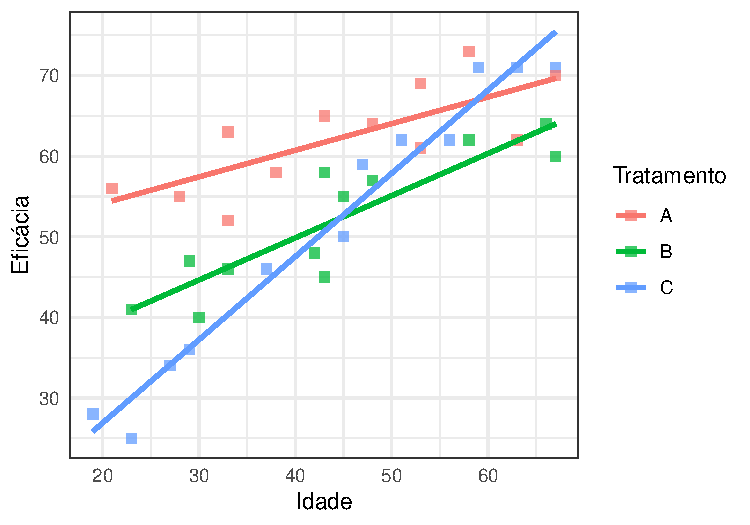
\includegraphics{lista2_files/figure-pdf/unnamed-chunk-20-1.pdf}

}

\caption{Curvas de regressão para modelo com interações.}

\end{figure}

Cabe recapitularmos que o grupo de referência é o tratamento C, o que
força a interpretação de que o intercepto \(\beta_0\) do modelo é o seu
efeito de tratamento isolado e \(\beta_1 \, x_{1i}\) se refere à
interação entre o tratamento C e a variável idade.

Podemos expressar então o modelo ajustado da seguinte forma:

\begin{align}
   \hat{y}_i &= \hat{\beta_0} + \hat{\beta_1} \, x_{1i} + \hat{\beta_2} \, x_{Ai} + \hat{\beta_3} \, x_{Bi} + \hat{\beta_4} \, x_{1i} \, x_{Ai} +\hat{\beta_5} \, x_{1i} \, x_{Bi} \nonumber \\
   \nonumber \\
   &= \begin{cases}
        \hat{\beta_0} + \hat{\beta_1} \, x_{1i}, \text{ se tratamento C} \\
        (\hat{\beta}_0 + \hat{\beta}_2) + (\hat{\beta}_1 + \hat{\beta}_4) x_{1i},  \text{ se tratamento A} \\
        (\hat{\beta}_0 + \hat{\beta}_3) + (\hat{\beta}_1 + \hat{\beta}_5) x_{1i},  \text{ se tratamento B}
      \end{cases} \nonumber \\
      \nonumber \\
  &= \begin{cases}
        6.21 + 1.03 \, x_{1i}, \text{ se tratamento C} \\
        47.51 + 0.33 \,  x_{1i},  \text{ se tratamento A} \\
        28.91 + 0.53 \,  x_{1i},  \text{ se tratamento B}
  \end{cases}\label{modelo_decomposto}
\end{align}

Em termos reais, o modelo sugere que há uma grande influência da idade
sobre a eficácia do tratamento C, enquanto essa influência é menor para
o tratamento B e menor ainda para o tratamento A.

\hypertarget{iii-tabela-anova}{%
\subsubsection{iii) Tabela ANOVA}\label{iii-tabela-anova}}

Finalmente, montamos a tabela de ANOVA do modelo. Em contraposição ao
modelo anterior, sem interações, vemos que uma pequena parcela da soma
de quadrados é atribuída aos resíduos. De fato, o coeficiente associado
ao efeito puro do tratamento B ainda explica muito pouco da variação do
modelo. No entanto, para que possamos considerar a interação Idade
\(\times\) Tratamento B, que testa significativamente para
\(H_a: \beta_j \neq 0\), mantemos o efeito puro.

\begin{longtable}[t]{lccccl}
\caption{Tabela ANOVA para o modelo linear com interações}\\
\toprule
Fonte de Var. & g.l. & SQ & QM & F & p-valor\\
\midrule
\endfirsthead
\caption[]{Tabela ANOVA para o modelo linear com interações \textit{(continued)}}\\
\toprule
Fonte de Var. & g.l. & SQ & QM & F & p-valor\\
\midrule
\endhead

\endfoot
\bottomrule
\endlastfoot
\cellcolor{gray!15}{idade} & \cellcolor{gray!15}{1} & \cellcolor{gray!15}{3424.432} & \cellcolor{gray!15}{3424.432} & \cellcolor{gray!15}{222.295} & \cellcolor{gray!15}{0.000}\\
A & 1 & 803.804 & 803.804 & 52.178 & 0.000\\
\cellcolor{gray!15}{B} & \cellcolor{gray!15}{1} & \cellcolor{gray!15}{1.189} & \cellcolor{gray!15}{1.189} & \cellcolor{gray!15}{0.077} & \cellcolor{gray!15}{0.783}\\
idade:A & 1 & 375.002 & 375.002 & 24.343 & 0.000\\
\cellcolor{gray!15}{idade:B} & \cellcolor{gray!15}{1} & \cellcolor{gray!15}{328.424} & \cellcolor{gray!15}{328.424} & \cellcolor{gray!15}{21.319} & \cellcolor{gray!15}{0.000}\\
Residuals & 30 & 462.148 & 15.405 & NA & NA\\*
\end{longtable}

\hypertarget{iv-anuxe1lise-completa-dos-resuxedduos-do-modelo}{%
\subsubsection{iv) Análise completa dos resíduos do
modelo}\label{iv-anuxe1lise-completa-dos-resuxedduos-do-modelo}}

Iniciamos a análise dos resíduos do modelo, supondo-se que
\(\varepsilon_i \sim N(0, \sigma^2)\), com testes de hipótese para
normalidade, heteroscedasticidade e independência dos dados. Avaliando
apenas os p-valores dos testes, não rejeitamos as hipóteses nulas e
podemos considerar a normalidade dos resíduos, constância da variância e
independência dos dados.

\begin{longtable}[t]{lcc}
\caption{Testes de hipótese para normalidade, heteroscedasticidade e independência.}\\
\toprule
Teste & Estatística de teste & p-valor\\
\midrule
\endfirsthead
\caption[]{Testes de hipótese para normalidade, heteroscedasticidade e independência. \textit{(continued)}}\\
\toprule
Teste & Estatística de teste & p-valor\\
\midrule
\endhead

\endfoot
\bottomrule
\endlastfoot
\cellcolor{gray!15}{Shapiro-Wilk normality test} & \cellcolor{gray!15}{0.963} & \cellcolor{gray!15}{0.263}\\
studentized Breusch-Pagan test & 2.996 & 0.701\\
\cellcolor{gray!15}{Durbin-Watson Test} & \cellcolor{gray!15}{1.633} & \cellcolor{gray!15}{0.214}\\*
\end{longtable}

Se analisarmos graficamente, notamos que os resíduos parecem
uniformemente distribuídos em torno de zero e com caudas mais pesadas no
QQplot. Isto favorece a hipótese de não normalidade, mas contradiz os
resultados do teste realizado. Verificaremos isso mais adiante.

Além disso, se avaliamos o gráfico de resíduos por sua alavancagem,
vemos que há alguns pontos com distância de Cook muito próxima a dois.
De fato, se utilizamos a função \texttt{stats::influence.measures()}
encontramos 4 pontos de alavancagem por algum dos critérios
apresentados. No entanto, nenhum deles está discrepante em ambos os
eixos, de modo que podemos considerá-los bons pontos de alavancagem.

\begin{figure}

{\centering 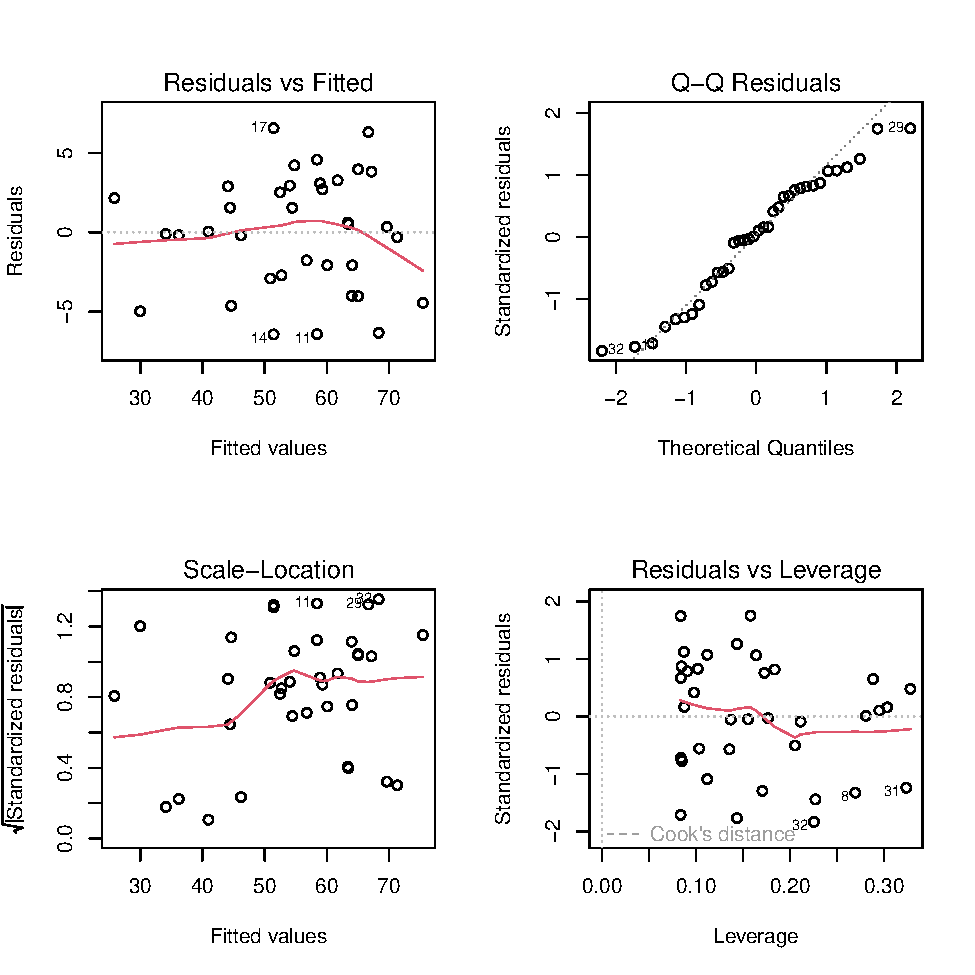
\includegraphics{lista2_files/figure-pdf/unnamed-chunk-21-1.pdf}

}

\end{figure}

Por fim, investigamos um pouco melhor os resíduos studentizados, gerando
um evenlopamento por bootstrap paramétrico\footnote{\url{https://github.com/cesar-galvao/modelos_lineares/blob/main/envelope_function.R}}.
De fato há pontos na borda da região designada como intervalo de
confiança. No entanto, considerando a distância deles ao intervalo e os
resultados dos demais testes, mantemos a afirmação de normalidade dos
resíduos e não são propostos mais ajustes ao modelo.

\begin{figure}

{\centering 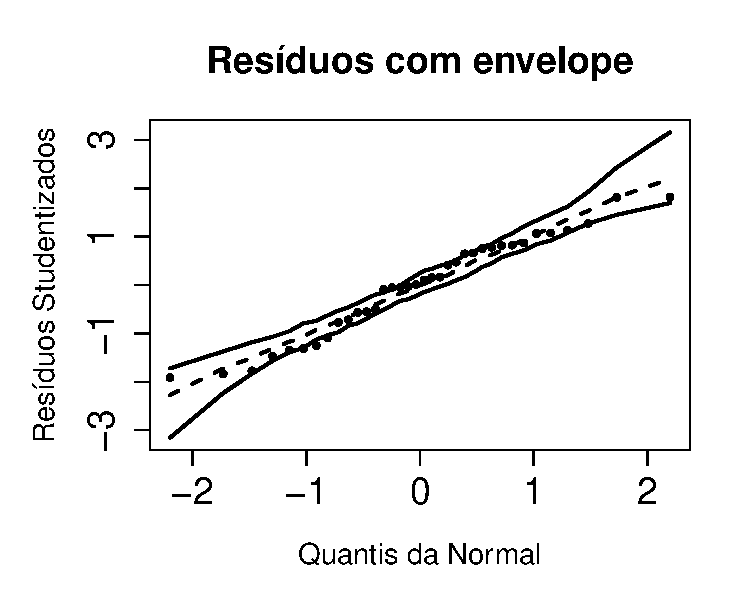
\includegraphics{lista2_files/figure-pdf/unnamed-chunk-22-1.pdf}

}

\end{figure}

\hypertarget{apuxeandice}{%
\section{Apêndice}\label{apuxeandice}}

Todo o projeto de composição deste documento pode ser encontrado aqui:
\url{https://github.com/cesar-galvao/mlg}

\begin{Shaded}
\begin{Highlighting}[]
\ControlFlowTok{if}\NormalTok{(}\SpecialCharTok{!}\NormalTok{(}\StringTok{"pacman"} \SpecialCharTok{\%in\%} \FunctionTok{installed.packages}\NormalTok{()))\{}\FunctionTok{install.packages}\NormalTok{(}\StringTok{"pacman"}\NormalTok{)\}}

\NormalTok{pacman}\SpecialCharTok{::}\FunctionTok{p\_load}\NormalTok{(tidyverse, tidymodels, kableExtra, corrplot, plotrix, lmtest, psych, car, phia, cowplot)}


\NormalTok{dados }\OtherTok{\textless{}{-}} \FunctionTok{read.table}\NormalTok{(}\StringTok{"dados lista 2/Q02\_data.txt"}\NormalTok{, }\AttributeTok{header=}\NormalTok{T)}

\NormalTok{dados }\SpecialCharTok{\%\textgreater{}\%}
  \FunctionTok{ggplot}\NormalTok{(}\FunctionTok{aes}\NormalTok{(eficacia))}\SpecialCharTok{+}
  \FunctionTok{geom\_histogram}\NormalTok{(}\AttributeTok{color =} \StringTok{"black"}\NormalTok{, }\AttributeTok{fill =} \StringTok{"gray"}\NormalTok{, }\AttributeTok{bins =} \DecValTok{10}\NormalTok{)}\SpecialCharTok{+}
  \FunctionTok{scale\_y\_continuous}\NormalTok{(}\AttributeTok{limits =} \FunctionTok{c}\NormalTok{(}\DecValTok{0}\NormalTok{, }\DecValTok{9}\NormalTok{),}
                     \AttributeTok{expand =} \FunctionTok{expansion}\NormalTok{(}\AttributeTok{mult =} \DecValTok{0}\NormalTok{, }\AttributeTok{add =} \DecValTok{0}\NormalTok{))}\SpecialCharTok{+}
  \FunctionTok{labs}\NormalTok{(}\AttributeTok{x =} \StringTok{"Eficácia"}\NormalTok{, }\AttributeTok{y =} \StringTok{""}\NormalTok{)}\SpecialCharTok{+}
  \FunctionTok{theme\_bw}\NormalTok{()}\SpecialCharTok{+}
  \FunctionTok{theme}\NormalTok{(}\AttributeTok{axis.ticks =} \FunctionTok{element\_blank}\NormalTok{())}

\NormalTok{dados }\SpecialCharTok{\%\textgreater{}\%}
  \FunctionTok{ggplot}\NormalTok{(}\FunctionTok{aes}\NormalTok{(eficacia, }\AttributeTok{fill =}\NormalTok{ tratamento))}\SpecialCharTok{+}
  \FunctionTok{geom\_histogram}\NormalTok{(}\AttributeTok{bins =} \DecValTok{10}\NormalTok{, }\AttributeTok{color =} \StringTok{"black"}\NormalTok{)}\SpecialCharTok{+}
  \FunctionTok{scale\_y\_continuous}\NormalTok{(}\AttributeTok{limits =} \FunctionTok{c}\NormalTok{(}\DecValTok{0}\NormalTok{, }\DecValTok{5}\NormalTok{),}
                     \AttributeTok{expand =} \FunctionTok{expansion}\NormalTok{(}\AttributeTok{mult =} \DecValTok{0}\NormalTok{, }\AttributeTok{add =} \DecValTok{0}\NormalTok{))}\SpecialCharTok{+}
  \FunctionTok{labs}\NormalTok{(}\AttributeTok{x =} \StringTok{"Eficácia"}\NormalTok{, }\AttributeTok{y =} \StringTok{""}\NormalTok{, }\AttributeTok{fill =} \StringTok{"Tratamento"}\NormalTok{)}\SpecialCharTok{+}
  \FunctionTok{theme\_bw}\NormalTok{()}\SpecialCharTok{+}
  \FunctionTok{theme}\NormalTok{(}\AttributeTok{axis.ticks =} \FunctionTok{element\_blank}\NormalTok{())}\SpecialCharTok{+}
  \FunctionTok{facet\_wrap}\NormalTok{(}\SpecialCharTok{\textasciitilde{}}\NormalTok{tratamento)}

\NormalTok{geral }\OtherTok{\textless{}{-}} \FunctionTok{ggplot}\NormalTok{(dados, }\FunctionTok{aes}\NormalTok{(}\AttributeTok{x =}\NormalTok{ idade, }\AttributeTok{y =}\NormalTok{ eficacia))}\SpecialCharTok{+}
  \FunctionTok{geom\_point}\NormalTok{(}\AttributeTok{shape =} \DecValTok{15}\NormalTok{, }\AttributeTok{size =} \DecValTok{2}\NormalTok{, }\AttributeTok{alpha =}\NormalTok{ .}\DecValTok{75}\NormalTok{)}\SpecialCharTok{+}
  \FunctionTok{geom\_smooth}\NormalTok{(}\AttributeTok{method =} \StringTok{"lm"}\NormalTok{, }\AttributeTok{se =} \ConstantTok{FALSE}\NormalTok{)}\SpecialCharTok{+}
  \FunctionTok{labs}\NormalTok{(}\AttributeTok{y =} \StringTok{"Eficácia"}\NormalTok{, }\AttributeTok{x =} \StringTok{"Idade"}\NormalTok{)}\SpecialCharTok{+}
  \FunctionTok{theme\_bw}\NormalTok{()}\SpecialCharTok{+}
  \FunctionTok{theme}\NormalTok{(}\AttributeTok{axis.ticks =} \FunctionTok{element\_blank}\NormalTok{())}

\NormalTok{trat }\OtherTok{\textless{}{-}} \FunctionTok{ggplot}\NormalTok{(dados, }\FunctionTok{aes}\NormalTok{(}\AttributeTok{x =}\NormalTok{ idade, }\AttributeTok{y =}\NormalTok{ eficacia, }\AttributeTok{color =}\NormalTok{ tratamento))}\SpecialCharTok{+}
  \FunctionTok{geom\_point}\NormalTok{(}\AttributeTok{shape =} \DecValTok{15}\NormalTok{, }\AttributeTok{size =} \DecValTok{2}\NormalTok{, }\AttributeTok{alpha =}\NormalTok{ .}\DecValTok{75}\NormalTok{)}\SpecialCharTok{+}
  \FunctionTok{labs}\NormalTok{(}\AttributeTok{y =} \StringTok{"Eficácia"}\NormalTok{, }\AttributeTok{x =} \StringTok{"Idade"}\NormalTok{)}\SpecialCharTok{+}
  \FunctionTok{theme\_bw}\NormalTok{()}\SpecialCharTok{+}
  \FunctionTok{theme}\NormalTok{(}\AttributeTok{axis.ticks =} \FunctionTok{element\_blank}\NormalTok{(),}
        \AttributeTok{legend.position =} \StringTok{"none"}\NormalTok{)}

\FunctionTok{plot\_grid}\NormalTok{(geral, trat)}

\CommentTok{\#da encoding à variavel tratamento}
\NormalTok{dados\_dummy }\OtherTok{\textless{}{-}}\NormalTok{ dados }\SpecialCharTok{\%\textgreater{}\%}
  \FunctionTok{mutate}\NormalTok{(}\AttributeTok{A =} \FunctionTok{if\_else}\NormalTok{(tratamento }\SpecialCharTok{==} \StringTok{"A"}\NormalTok{, }\DecValTok{1}\NormalTok{, }\DecValTok{0}\NormalTok{),}
         \AttributeTok{B =} \FunctionTok{if\_else}\NormalTok{(tratamento }\SpecialCharTok{==} \StringTok{"B"}\NormalTok{, }\DecValTok{1}\NormalTok{, }\DecValTok{0}\NormalTok{)) }\SpecialCharTok{\%\textgreater{}\%}
\NormalTok{  dplyr}\SpecialCharTok{::}\FunctionTok{select}\NormalTok{(}\SpecialCharTok{{-}}\NormalTok{tratamento)}

\CommentTok{\#monta fit aditivo do modelo}
\NormalTok{fit\_depressao }\OtherTok{\textless{}{-}} \FunctionTok{lm}\NormalTok{(eficacia }\SpecialCharTok{\textasciitilde{}}\NormalTok{ (.), }\AttributeTok{data =}\NormalTok{ dados\_dummy)}

\CommentTok{\#tabela do modelo}
\NormalTok{fit\_depressao }\SpecialCharTok{\%\textgreater{}\%}
  \FunctionTok{summary}\NormalTok{() }\SpecialCharTok{\%\textgreater{}\%} 
  \FunctionTok{tidy}\NormalTok{()}

\FunctionTok{anova}\NormalTok{(fit\_depressao) }\SpecialCharTok{\%\textgreater{}\%}
  \FunctionTok{tidy}\NormalTok{()}

\NormalTok{fit\_depressao\_intera }\OtherTok{\textless{}{-}} \FunctionTok{lm}\NormalTok{(eficacia }\SpecialCharTok{\textasciitilde{}}\NormalTok{ (.) }\SpecialCharTok{+}\NormalTok{ idade}\SpecialCharTok{*}\NormalTok{A }\SpecialCharTok{+}\NormalTok{ idade}\SpecialCharTok{*}\NormalTok{B, }\AttributeTok{data =}\NormalTok{ dados\_dummy)}

\NormalTok{fit\_depressao\_intera }\SpecialCharTok{\%\textgreater{}\%}
  \FunctionTok{summary}\NormalTok{() }\SpecialCharTok{\%\textgreater{}\%} 
  \FunctionTok{tidy}\NormalTok{()}

\NormalTok{nomes }\OtherTok{\textless{}{-}} \FunctionTok{row.names}\NormalTok{(}\FunctionTok{confint}\NormalTok{(fit\_depressao\_intera, }\AttributeTok{level=}\FloatTok{0.95}\NormalTok{))}

\NormalTok{tabela }\OtherTok{\textless{}{-}} \FunctionTok{confint}\NormalTok{(fit\_depressao\_intera, }\AttributeTok{level=}\FloatTok{0.95}\NormalTok{) }\SpecialCharTok{\%\textgreater{}\%} 
  \FunctionTok{as\_tibble}\NormalTok{() }\SpecialCharTok{\%\textgreater{}\%}
  \FunctionTok{mutate}\NormalTok{(}\AttributeTok{Estimador =}\NormalTok{ nomes) }\SpecialCharTok{\%\textgreater{}\%}
\NormalTok{  dplyr}\SpecialCharTok{::}\FunctionTok{select}\NormalTok{(Estimador, }\FunctionTok{everything}\NormalTok{()) }

\FunctionTok{ggplot}\NormalTok{(dados, }\FunctionTok{aes}\NormalTok{(}\AttributeTok{x =}\NormalTok{ idade, }\AttributeTok{y =}\NormalTok{ eficacia, }\AttributeTok{color =}\NormalTok{ tratamento))}\SpecialCharTok{+}
  \FunctionTok{geom\_point}\NormalTok{(}\AttributeTok{shape =} \DecValTok{15}\NormalTok{, }\AttributeTok{size =} \DecValTok{2}\NormalTok{, }\AttributeTok{alpha =}\NormalTok{ .}\DecValTok{75}\NormalTok{)}\SpecialCharTok{+}
  \FunctionTok{geom\_smooth}\NormalTok{(}\AttributeTok{method =} \StringTok{"lm"}\NormalTok{, }\AttributeTok{se =} \ConstantTok{FALSE}\NormalTok{)}\SpecialCharTok{+}
  \FunctionTok{labs}\NormalTok{(}\AttributeTok{y =} \StringTok{"Eficácia"}\NormalTok{, }\AttributeTok{x =} \StringTok{"Idade"}\NormalTok{, }\AttributeTok{color =} \StringTok{"Tratamento"}\NormalTok{)}\SpecialCharTok{+}
  \FunctionTok{theme\_bw}\NormalTok{()}\SpecialCharTok{+}
  \FunctionTok{theme}\NormalTok{(}\AttributeTok{axis.ticks =} \FunctionTok{element\_blank}\NormalTok{())}

\FunctionTok{anova}\NormalTok{(fit\_depressao\_intera) }\SpecialCharTok{\%\textgreater{}\%}
  \FunctionTok{tidy}\NormalTok{()}

\FunctionTok{bind\_rows}\NormalTok{(}
  \DocumentationTok{\#\# Perform the normal Shapiro{-}Wilk test for the residuals}
  \FunctionTok{shapiro.test}\NormalTok{(}\FunctionTok{residuals}\NormalTok{(fit\_depressao\_intera)) }\SpecialCharTok{\%\textgreater{}\%} \FunctionTok{tidy}\NormalTok{(),}
  
  \DocumentationTok{\#\# Perform breush{-}pagan test for hetereocedascity}
\NormalTok{  (}\FunctionTok{bptest}\NormalTok{(fit\_depressao\_intera) }\SpecialCharTok{\%\textgreater{}\%} \FunctionTok{tidy}\NormalTok{())[, }\FunctionTok{c}\NormalTok{(}\DecValTok{1}\NormalTok{, }\DecValTok{2}\NormalTok{, }\DecValTok{4}\NormalTok{)],}
  
  \DocumentationTok{\#\# Perform Durbin{-}Watson test for Independence}
\NormalTok{  (}\FunctionTok{durbinWatsonTest}\NormalTok{(fit\_depressao\_intera) }\SpecialCharTok{\%\textgreater{}\%} \FunctionTok{tidy}\NormalTok{())[,}\FunctionTok{c}\NormalTok{(}\DecValTok{1}\NormalTok{, }\DecValTok{2}\NormalTok{, }\DecValTok{4}\NormalTok{)]}
\NormalTok{) }\SpecialCharTok{\%\textgreater{}\%}
\NormalTok{  dplyr}\SpecialCharTok{::}\FunctionTok{select}\NormalTok{(method, }\FunctionTok{everything}\NormalTok{())}

\FunctionTok{par}\NormalTok{(}\AttributeTok{mfrow=}\FunctionTok{c}\NormalTok{(}\DecValTok{2}\NormalTok{,}\DecValTok{2}\NormalTok{))}
\FunctionTok{plot}\NormalTok{(fit\_depressao\_intera)}

\FunctionTok{source}\NormalTok{(}\StringTok{"dados lista 2/envelope\_function.R"}\NormalTok{)}
\FunctionTok{envelope\_LR}\NormalTok{(fit\_depressao\_intera, }\AttributeTok{OLS =}\NormalTok{ T, }\AttributeTok{main.title =} \StringTok{"Resíduos com envelope"}\NormalTok{)}
\end{Highlighting}
\end{Shaded}




\end{document}
